% AASTeX v6.2
%\documentclass[preprint]{aastex62}

% ApJ Format
\documentclass[iop,revtex4,twocolumn,apj,numberedappendix,appendixfloats]{emulateapj}
\usepackage{apjfonts}
% Hyperlinks & Bookmarks
\usepackage[pagebackref=false,colorlinks=true,citecolor=blue,linkcolor=blue,breaklinks=true,bookmarks=true]{hyperref}
\usepackage{amsmath}
\usepackage{comment}

% Units
\newcommand{\kms}{km~s$^{-1}$}
\newcommand{\msun}{$M_{\odot}$}
\newcommand{\msunyr}{$M_{\odot}~{\rm yr}^{-1}$}
\newcommand{\lsun}{$L_{\odot}$}
\newcommand{\ergs}{erg~s$^{-1}$}
\newcommand{\cmsq}{cm$^{-2}$}
\newcommand{\um}{$\mu$m}
\newcommand{\uJy}{$\mu$Jy}
\newcommand{\sqdeg}{deg$^2$}
\newcommand{\lx}{$L_{\rm X}$}
\newcommand{\lmir}{$L_{\rm 12\mu m}$}
\newcommand{\loiii}{$L_{\rm [OIII]}$}
% Emission lines
\newcommand{\Ha}{H$\alpha$}
\newcommand{\Hb}{H$\beta$}
\newcommand{\OII}{[O\,{\sc ii}]}
\newcommand{\OIIlam}{[O\,{\sc ii}]\,$\lambda$3727}
\newcommand{\SII}{[S\,{\sc ii}]}
\newcommand{\OIII}{[O\,{\sc iii}]}
\newcommand{\OIIIlam}{[O\,{\sc iii}]\,$\lambda$5007}
\newcommand{\NII}{[N\,{\sc ii}]}
\newcommand{\NeIII}{[Ne\,{\sc iii}]}
% special 
\newcommand{\nod}{\nodata}

\newcommand{\angstrom}{\mbox{\normalfont\AA}}
\newcommand{\reff}{$R_{\rm eff}$}
\newcommand{\ewha}{EW(H$\alpha$)}
\newcommand{\logm}{log({\it M}/M$_{\odot}$)}
%\newcommand{\arcsec}{\prime\prime}
\newcommand{\simard}{Simard+11}

% citations
\defcitealias{Fu18}{Paper I} 

\usepackage{epstopdf}

\begin{document}

\title{SDSS-IV MaNGA: Radial Profiles of Specific Star Formation Rate in Nearby Interacting Galaxies}

\author{
Joshua L. Steffen\altaffilmark{1}, 
Hai Fu\altaffilmark{1}, and 
MaNGA Team 
}
\altaffiltext{1}{Department of Physics \& Astronomy, The University of Iowa, 203 Van Allen Hall, Iowa City, IA 52242}

\begin{abstract}
We study the spatial profile of the star formation rate (SFR) in a sample of 202 interacting galaxies within the MaNGA (Mapping Nearby Galaxies at Apache Point Observatory) survey. We find that the specific star formation rate (sSFR) is centrally enhanced in the interacting galaxies by $\sim$0.25 $\pm$ 0.1 but that there is no enhancement or suppression in their disks. We further investigate how these profiles behave as a function of stellar mass, mass ratio, and projected separation. We find that the sSFR profiles are unaffected by the stellar masses of the interacting galaxies; however, they are affected by the mass ratio between the galaxies where the galaxies with the smallest mass ratio feature the largest enhancement. We also find that, in pairs with large mass ratios ($|\Delta$log(M)$|$ $=$ 0.5 $-$ 1.5), the less massive galaxy of the pair has slightly higher levels of sSFR enhancement, $\sim$0.1 dex. We also find that the level of sSFR enhancement increases with closer projected separations; however, the closest pairs, $\le$5 kpc, show no signs of sSFR enhancement/suppression. We suspect that these close pairs are merging galaxies which have passed their first pericenter, but the merger induced gas-inflows have yet to reach the centers of the galaxies. We also set a simple model for the future mass growth of the galaxies due to the merger induced star formation. We predict that the paired galaxies in our sample will see a mass growth rate which is XX$\times$ higher than secular mass growth. 
\end{abstract}

\keywords{galaxies: active --- galaxies: nuclei --- galaxies: interactions}

%%%%%%%%%%%%%%%%%%%%%%%%%%%%%%%%%%%%%%%%%%%%%%%%%%%%
\section{Introduction}\label{sec:intro}

%%%Galaxy Evolution%%%
In the $\Lambda$CDM model, galaxy evolution is a hierarchical process. Over the lifetime of the universe, smaller galaxies have iteratively merged forming more massive galaxies. In fact, cosmological hydrodynamical simulations have shown that repeated merger events may be responsible for as much as $\sim$60\% of stellar mass in massive galaxies like M87 (e.g. \citet{Rodriguez-Gomez:2016}; \citet{Pillepich:2018}). 

%%%Simulations%%%
The internal dynamics of these interacting galaxies were first modeled in the seminal work, \citet{Toomre:1972}. Since then, hydrodynamical simulations have expanded upon the N-body simulations of \citet{Toomre:1972} by modeling gas-dynamics within the galaxies. These simulations show how barred structures develop within the disks of the interacting galaxies due to the tidal torques between them \citep{Barnes:1991}. As the bars form, the gases within the galaxy's disk lose angular momentum and get funneled into the centers of the galaxies. 

When the gas-inflows impact upon the gases in the nucleus of galaxy a burst of new star formation in triggered \citep{Barnes:1996, Mihos:1996}. These gas inflows will also bring metal-poor gases from the disk into the center of the galaxy which can dilute the central metallicity \citep{Rupke:2010, Perez:2011, Scudder:2012}. The gas-inflows may also be able to make it into very center of the galaxy and trigger supermassive black hole (SMBH) accretion \citep{Capelo:2017}. 

%%%Observations%%%
Centrally enhanced star formation has also been observed in large spectroscopic surveys including; CfA2  \citep{Barton:2000, Woods:2006}, 2dF \citep{Lambas:2003}, AEGIS \citep{Lin:2007}, SDSS \citep{Ellison:2008}, COSMOS \citep{Kartaltepe:2007,Xu:2012}, PRIMUS \citep{Wong:2011}, and GAMA \citep{Robotham:2014}.

This star formation enhancement increases with closer projected separations between the two galaxies \citep{Ellison:2008, Scudder:2012} but has still shown to be detectable at projected separations of 150 kpc \citep{Patton:2013}. The level of the star formation enhancement also increases with smaller stellar mass ratios, $|\Delta log {\it M} |$, between the two galaxies \citep{Ellison:2008}. 

%%%Integral Field Spectroscopy%%%
With the recent large integral field spectroscopic (IFS) surveys, interacting galaxies can be studied with unprecedented spatial detail. Where previous spectroscopic surveys were limited to the nucleus of the interacting galaxies, the new IFS surveys will be able to study both the nuclei and the disks of the interacting galaxies. 

The IFS surveys, CALIFA\footnote{Calar Alto Legacy Integral Field Area} and MaNGA\footnote{Mapping Nearby Galaxies at Apache Point Observatory}, have already been used to study the SFR of interacting galaxies in merging galaxies. The SFR was found to be centrally enhanced by a factor of 2$-$3$\times$ \citep{Barrera-Ballesteros:2015, Pan:2019}, which is in agreement with previous single-fiber spectroscopic surveys. These surveys also studied the SFR in the disk of the paired galaxies; however, there is a discrepancy between the results. \citet{Barrera-Ballesteros:2015} found a suppression to the SFR of $\sim$0.74$\times$ while \citet{Pan:2019} found an enhancement of 1.22$-$1.58$\times$. 

The MaNGA survey has also been used to study the radial profiles of SFR in post merger galaxies, which are the galaxies which have recently coalesced. The post merger galaxies showed a central enhancement to the SFR surface density of 2.5$\times$ and an enhancement in their disks of 1.26$\times$ \citep{Thorp:2019}.

%%%Purpose%%%
In our previous work, \citet{Fu:2018}, we built a sample of paired galaxies in the MaNGA survey where both components of the pair were contained within field of view of a single IFU. We found that approximately 5.7\% of the MaNGA galaxies have a companion galaxies contained with the IFU. In this work, we will use a version of this sample updated for the recent MaNGA Data Release 16 (DR16) and further supplement this with a sample of companion galaxies identified outside the field of view of the IFUs. 

In this work we will expand upon the previous works by studying how the spatial profile of SFR behaves as a function of the stellar mass of the paired galaxy, the mass ratio between the galaxy pairs, and the projected separation between the galaxies. We will also model how the merger-induced star formation will affect the future mass growth of the interacting galaxies. 

% Organization
This paper is organized as follows; in Section \ref{sec:data} we will discuss the detail of the MaNGA survey, in Section \ref{sec:analysis} we will discuss how we extract emission lines from the MaNGA survey and how we calculate the star formation from them, in Section \ref{sec:pair} we discuss the construction of our pair sample, in Section \ref{sec:control} we discuss the construction of our control sample, in Section \ref{sec:radial} we build the radial profiles for the pair and control galaxies, in Section \ref{sec:results} we discuss the results of the survey, in Section \ref{sec:discussion} we discuss our results in the context of other surveys, and in Section \ref{sec:sum} we summarize and conclude the work. 

%%%%%%%%%%%%%%%%%%%%%%%%%%%%%%%%%%%%%%%%%%%%%%%%%%%%
\section{Data}\label{sec:data}

MaNGA is an a IFS survey based at Apache Point Observatory (APO) which used the SDSS 2.5 meter telescope along with two dual-channel BOSS spectrographs. MaNGA captures spectra through 17 integral field units (IFUs) with variable numbers of fibers; 19, 37, 61, 91, and 127 fibers covering 12.5\arcsec, 17.5\arcsec, 22.5\arcsec, 27.5\arcsec, and 32.5\arcsec on the sky respectively. MaNGA is an optical survey with a spectral coverage of 3600$-$10,300 \AA with a resolution of R $\sim$ 2000 and a median spectra coverage of 2.5\arcsec FWHM \citep{Bundy:2015}. 

MaNGA targets galaxies from a subset of 41,154 galaxies with from the NASA-Sloan Atlas (NSA) with a redshift range of 0.01 $<$ z $<$ 0.15 and a luminosity range of -17.7 $<$ $\mathcal{M_{\rm i}}$ $<$ -24.0, where $\mathcal{M_{\rm i}}$ is the rest frame i-band magnitude within the NSA survey's elliptical Petrosian apertures. MaNGA plans to cover 10,000 galaxies with a flat stellar mass distribution at two spatial coverages, 1.5 \reff\ and 2.5 \reff\ (where \reff\ is the radius which contains 50\% of the galaxy's total light). In this work we use the data from the internal data release, MPL-8, which covers 6142 unique galaxies. 

The MaNGA sample is split into three subsamples; the Primary Sample, Secondary Sample, and Color-Enhanced Sample. The Primary sample contains the galaxies which are covered out to 1.5 \reff\ and makes up 47\% of the survey. The Secondary contains the galaxies which are covered out to 2.5 \reff\ and makes up 37\% of the survey. The Color-Enhanced sample is designed to select rarer galaxy types with a spatial coverage of 2.5 \reff\ and makes up 16\% of the survey. 

Because of the survey's flat stellar mass distribution and uniform spatial coverage, these samples have a unique ``banana" shaped distribution in redshift and luminosity, see Figure \ref{fig:Mi-z}. Because the Secondary and Color-Enhanced samples use a wider spatial coverage than the Primary sample, the Secondary and Color-Enhanced Samples will posses galaxies of higher redshifts than galaxies at the same stellar masses in the Primary sample. 

%%% NSA and Simard+11
We further use photometric data from the NSA catalog and \citet{Simard:2011} (from now on \simard). We use the r-band elliptical Petrosian apertures from the NSA catalog and the r-band elliptical S\'ersic apertures from \simard\ to quantify the geometry of the outside-IFU and inside-IFU samples respectively. We further use the total stellar masses extracted from these apertures to quantify the total stellar masses of the galaxies, the NSA catalog contains their own calculation for stellar mass and we use the stellar mass calculation from \citet{Mendel:2014} for the \simard\ apertures.

%%%%%%%%%%%%%%%%%%%%%%%%%%%%%%%%%%%%%%%%%%%%%%%%%%%%
\section{Analysis}\label{sec:analysis}
\subsection{Emission Lines}

%%%%%%%%%%%%%%%%%%%%%%%%%%%%%%%%%%%%%%%%%%%%%%
\begin{figure*}
\centering
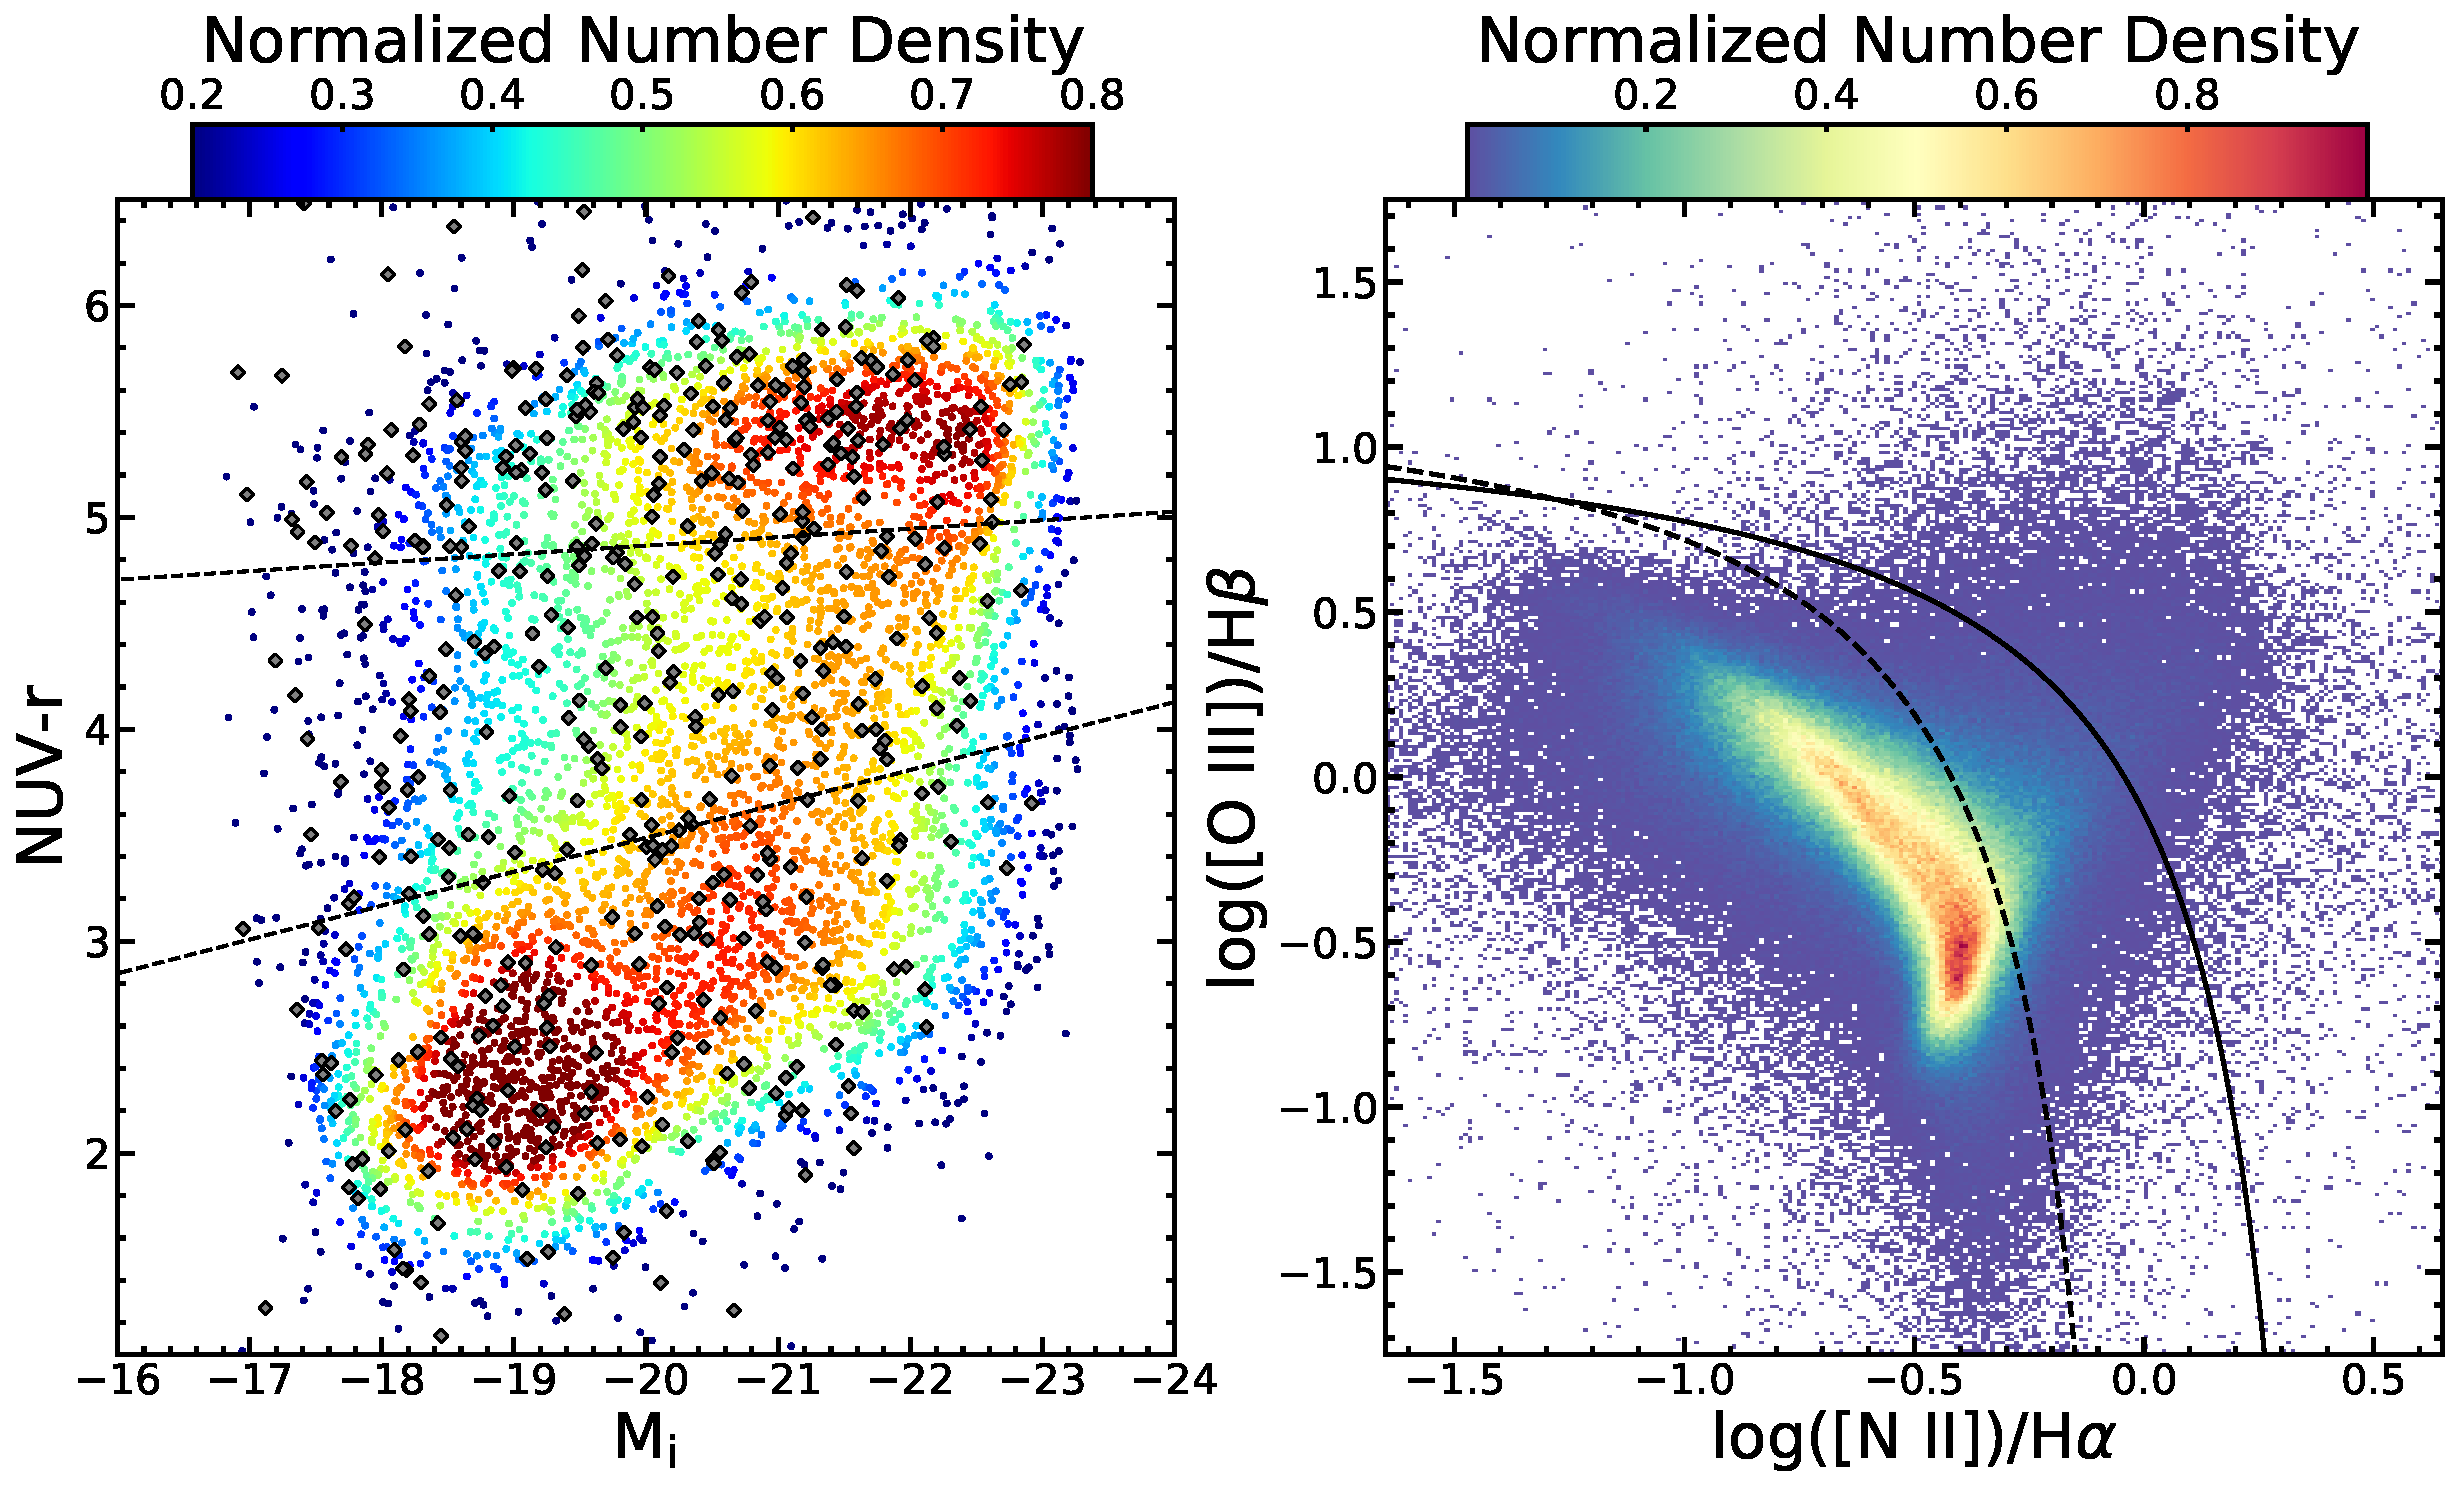
\includegraphics[width=\linewidth]{fig/bpt-cmd.pdf}
\caption[]{\textbf{Left:} Color-magnitude diagram for MaNGA galaxies ({\it colored circles}). The color of the symbol reflects the local density around each data point in this color-magnitude plane, as indicated by the color bar on the top. The MaNGA galaxies with close companions are marked with {\it grey diamonds}. From top to bottom, the dashed lines divide the sample into red sequence, green valley, and blue cloud. The star-forming galaxy sample used in this paper are the galaxies below the lower dividing line. \textbf{Right:} The 2-D histogram showing the BPT classification \citep{Baldwin:1981} of individual spaxels within our star-forming control and pair samples. The color of each bin represents the number density of spaxels, normalized to one. The solid black line represents the theoretically determined maximum starburst line of \citet{Kewley:2001} and the dashed black line is the analytical \citet{Kauffmann:2003} line. This shows the capability of the CMD to select star-forming galaxies as most of the spaxels within the selected galaxies fall beneath the starburst line.}
\label{fig:cmd}
\end{figure*}
%%%%%%%%%%%%%%%%%%%%%%%%%%%%%%%%%%%%%%%%%%%%%%

%%% SPFIT
We use our own {\sc IDL} based spectral fitting code, {\sc SPFIT}, to model the spectra from the MaNGA datacubes. {\sc SPFIT} simultaneously fits emission lines and the stellar continuum with the Levenberg-Marquardt nonlinear least-squares minimization algorithm \citep{Fu:2018}. Emission line are parameterized as a Gauss-Hermite series and the stellar continuum is the sum of simple stellar populations (SSPs) convolved with the line-of-sight velocity distribution (LOSVD). The algorithm provides us with measurements of emission line fluxes, equivalent widths, velocities, and velocity dispersions of 19 emission lines and measurements of stellar masses, ages, [Fe/H], and kinematics of the stellar populations. 

%%% Reddening
We use the extinction curve from \citet{Cardelli:1989} with updated coefficients from \citet{ODonnell:1994}. The extinction in parameterized as R$_V$ $\equiv$ A$_V$/E(B$-$V) $=$ 3.1 where we estimate the value of the V-band extinction, A$_V$, by comparing the H$\alpha$/H$\beta$ to the expected value of 2.85 for case-B recombination. We apply the extinction correction to all of the extracted emission lines.

\subsection{Star Formation Rates}
We classify galaxies as star forming using both the color-magnitude diagram (CMD) and the BPT diagram \citep{Baldwin:1981}. We show the CMD in Figure \ref{fig:cmd} along with demarcation lines which separate the blue cloud, red sequence, and green valley. We established the demarcation lines by collapsing the CMD to a color histogram for each of the three regions and then varied the slopes between the regions until we found the slopes which best fit the data. These demarcation lines are;

\begin{equation}\label{eq:blue}
NUV-r = 3.1682 - 0.16 (M_i+18)
\end{equation}
\begin{equation}\label{eq:red}
NUV-r = 4.7866 - 0.04 (M_i+18)
\end{equation}

Where NUV$-$r is the color and M$_i$ is the i-band magnitude. 

The BPT diagnostic uses emission line ratios to separate ionization sources, star formation and active galactic nuclei (AGN). The two ionization sources can be separated by either the theoretical maximum starburst line from \citet{Kewley:2001} or the analytically fitted line from \citet{Kauffmann:2003}, given below in Equations \ref{eq:kewley} and \ref{eq:kauffmann} respectively.

\begin{equation}\label{eq:kewley}
\rm{log\Big(\frac{[O\,\textsc{iii}]\lambda 5007}{H\beta}\Big) = \frac{0.61}{log([N\,\textsc{ii}]\lambda 6584 / H\alpha) - 0.47} + 1.19}
\end{equation}
\begin{equation}\label{eq:kauffmann}
\rm{log\Big(\frac{[O\,\textsc{iii}]\lambda 5007}{H\beta}\Big) = \frac{0.61}{log([N\,\textsc{ii}]\lambda 6584 / H\alpha) - 0.05} + 1.3}
\end{equation}

Where \OIII$\lambda$5007, H$\beta$, \NII$\lambda$6584, and H$\alpha$ are emission line fluxes extracted from the spectra within the inner 2 arcseconds of the galaxies. It has also been shown that hot low mass evolved stars (HOLMES) in retired galaxies can mimic HII regions and AGN on the BPT diagram \citep{Stasinska:2008}. We apply an H$\alpha$ equivalent width (EW) cut of \ewha\ $>$ 3\angstrom to remove these retired galaxies \citet{Cid-Fernandes:2011}. In this work, we define star forming galaxies as those which are on the blue cloud in the CMD and which is below the \citet{Kewley:2001} on the BPT diagram.

We measure the SFR from the H$\alpha$ luminosity, L$_{H\alpha}$. The H$\alpha$ luminosity is calculated from the flux of the H$\alpha$ emission line. We use the SFR formula, Equation \ref{eq:sfr}, from \citet{Murphy:2011} which uses a Kroupa IMF, Solar metallicity, a constant SFR at an age of 100 Myr, and Case-B recombination. 

\begin{equation}\label{eq:sfr}
\frac{\rm{SFR}}{M_{\odot} \, \rm{yr^{-1}}} = \frac{L_{H\alpha}}{1.86 \times 10^{41}\, \rm{erg\,s}^{-1}}
\end{equation}

We normalize the SFR by the local stellar mass (the stellar mass contained with a given spaxel), calculated from SPFIT, giving us the specific star formation rate (sSFR). 

\begin{equation}
sSFR = \frac{SFR}{M^*}
\end{equation}

This will allow us to compare the SFR in high mass regions, like the centers of the galaxies, to the SFR lower mass regions, like the disk of the galaxies.

%%%%%%%%%%%%%%%%%%%%%%%%%%%%%%%%%%%%%%%%%%%%%%%%%%%%
\section{Pair Sample}\label{sec:pair}

\subsection{Inside-IFU Sample}\label{sec:inside}
In our previous work, \citet{Fu:2018}, we showed that $\sim$5.7\% of the MaNGA observations have at least one companion galaxy within the field of view of the IFU. In this work we use a refined pair identification process which is also expanded for the most recent internal data release, MPL-8.

We use SDSS photometric objects to create a catalog of objects within the fields of view of the MaNGA IFUs. The extract their spectra from the MaNGA datacubes through a 1\arcsec aperture and fit the spectra with {\sc SPFIT}. The spectra is then sorted into different categories; ``good" galaxy spectra, broad-line AGN, foreground star, foreground/background galaxies, or poor S/N objects. The ``good" galaxy spectra are the objects whose spectra is well modeled by {\sc SPFIT} at the target galaxy's redshift, whether it is the target galaxies itself or a nearby companion galaxy. This means that the companion galaxy can be within $\pm$3000 km s$^{-1}$ of the MaNGA target. We found 6573 ``good" objects, 57 broad-line AGN, 836 foreground stars, 319 foreground/background galaxies, and 1546 objects with poor S/N. 

From the 6573 galaxies with good spectra, 404 of the MaNGA IFUs have multiple objects within the IFU and within a relative velocity of $\Delta$v $<$ 500 km s$^{-1}$. 124 of the galaxies are star forming galaxies (SFGs). Finally, 41 SFGs are covered by \simard\ and \citet{Mendel:2014}. 

Some of the galaxies in our sample have multiple companions. From the whole set of 404 IFUs, there are 327 pairs, 67 triplets, 7 quadruplets, and 1 quintuplet.  

We characterize the geometry of the inside-IFU galaxies with the r-band elliptical S\'ersic apertures and we characterize the total stellar mass of the galaxies with the stellar masses from \citet{Mendel:2014}


\subsection{Outside-IFU Sample}\label{sec:outside}

The second pairs sample is the outside-IFU pairs sample. This sample includes MaNGA galaxies which have companion galaxies found outside the field of view of its IFU. We identify these external pair from the NSA catalog. We select galaxies which are within a projected separation, r$_p$ $<$ 50 kpc, and within a relative velocity, $\Delta$v $<$ 500 km s$^{-1}$. 

The NSA catalog contains 641,409 galaxies from which we find 509 galaxies which are paired to MaNGA targets. MaNGA targets which have both an inside-IFU and an outside-IFU pair are left to the inside-IFU sample. After restricting the sample to SFGs, we have 161 MaNGA targets with paired galaxies outside of the IFU.

We use the r-band elliptical Petrosian apertures from the NSA catalog to describe the geometry of the galaxies in the outside-IFU sample. We also use the stellar masses from the NSA catalog for the total stellar mass of the galaxies. 

%%%%%%%%%%%%%%%%%%%%%%%%%%%%%%%%%%%%%%%%%%%%%%%%%%%%
\section{Control Sample}\label{sec:control}
We build a sample of isolated control galaxies from the remaining MaNGA galaxies. Selecting the MaNGA galaxies which have no spectroscopic companions within r$_p$ $<$ 50 kpc and $\Delta$v $<$ 500 km s$^{-1}$ either inside or outside of the IFU. This gives us a set of 1862 SFGs and 1598 SFGs which are covered by both \simard\ and \citet{Mendel:2014}. 

The SFR in galaxies has been shown to be dependent on both stellar mass and redshift \citep{Noeske:2007}. To account for this we will need to match pairs with similar mass and redshift controls. To do this we build a subset of 20 control galaxies for each paired galaxy. 

First we select every control galaxy which is within a stellar mass of 0.1 dex and within in same MaNGA subsample, i.e. the Primary or Secondary sample. Knowing that MaNGA has a tight ``banana" shaped distribution in stellar mass and redshift, imposing the stellar mass cut and the MaNGA subsample cut will effectively set a $\sim$0.025 dex redshift cut.

We then downselect the control subset down to 20 controls using a random number generator so that each paired galaxies has the same number of selected controls. In the few cases where a paired galaxy fails to find at least 20 control galaxies, we iteratively expand the stellar mass limits by 0.1 dex until a set of 20 control galaxies can be made. A small set of paired required extra iterations to find 20 controls; 8 paired galaxies need an extra iteration, 1 paired galaxy need two extra iterations, and 1 paired galaxy needed three iterations. \\

The control galaxies will be treated using both the \simard\ aperture and \citet{Mendel:2014} masses when comparing them to the inside-IFU sample and the NSA apertures and masses when comparing them to the outside-IFU sample. 

%%%%%%%%%%%%%%%%%%%%%%%%%%%%%%%%%%%%%%%%%%%%%%%%%%%%
\section{Radial Profiles}\label{sec:radial}

As mentioned in Sections \ref{sec:pair} and \ref{sec:control} we use the r-band elliptical Petrosian apertures from the NSA catalog and the r-band S\'ersic apertures from \simard to define the geometries of the galaxies. We calculate the inclination angle, {\it i}, of the galaxies using the major-to-minor axis ratios from the elliptical apertures;

\begin{equation}
{\rm cos^2}(i) = \frac{(b/a)^2 - q^2}{1 - q^2}
\end{equation}

The inclination angle is used to deproject the geometries of the galaxies. We use our catalog of photometric objects and the \simard\ catalog to mask foregournd/background objects. Objects in our photometric catalog are masked out with a 2\arcsec\ circular aperture and the galaxies from \simard\ are masked out with a 2.0 \reff\ elliptical aperture, using the r-band S\'ersic apertures from the catalog. 

The distance to each of the spaxels from the center of the MaNGA targets is calculated using the 50\% half light radius to scale the galaxies. The spaxels are binned into radius increments of 0.1 \reff\ from 0.0$-$2.4\reff. Within each radius bin we take the median of the specific star formation rate. The profiles' errors are the standard error of the mean of the data within each radius bin. We create one of these individual averaged radial profiles for every MaNGA galaxy. 

We then construct difference profiles between the paired galaxies and the control galaxies. As mentioned in Section \ref{sec:control}, a paired galaxy is matched to 20 similar control galaxies. We take the individual averaged profiles of the control galaxies and take the median value of the profiles at each radius bin giving us a ``stacked" profile of control galaxies. The error of the profile is the standard error of the mean of the individual profiles. We also take into account the error associated with the random selection of controls using a bootstrapping method to quantify the variation in the values of stacked profile over 1000 iterations. The difference profile is then the difference between a single paired galaxy's profile and the stacked profile in log space (this means that the difference profiles are ratios in linear space). This is done for each of the 202 galaxy pairs. 


%%%%%%%%%%%%%%%%%%%%%%%%%%%%%%%%%%%%%%%%%%%%%%%%%%%%
\section{Results}\label{sec:results}
%%%%%%%%%%%%%%%%%%%%%%%%%%%%%%%%%%%%%%%%%%%%%%
\begin{figure}
\centering
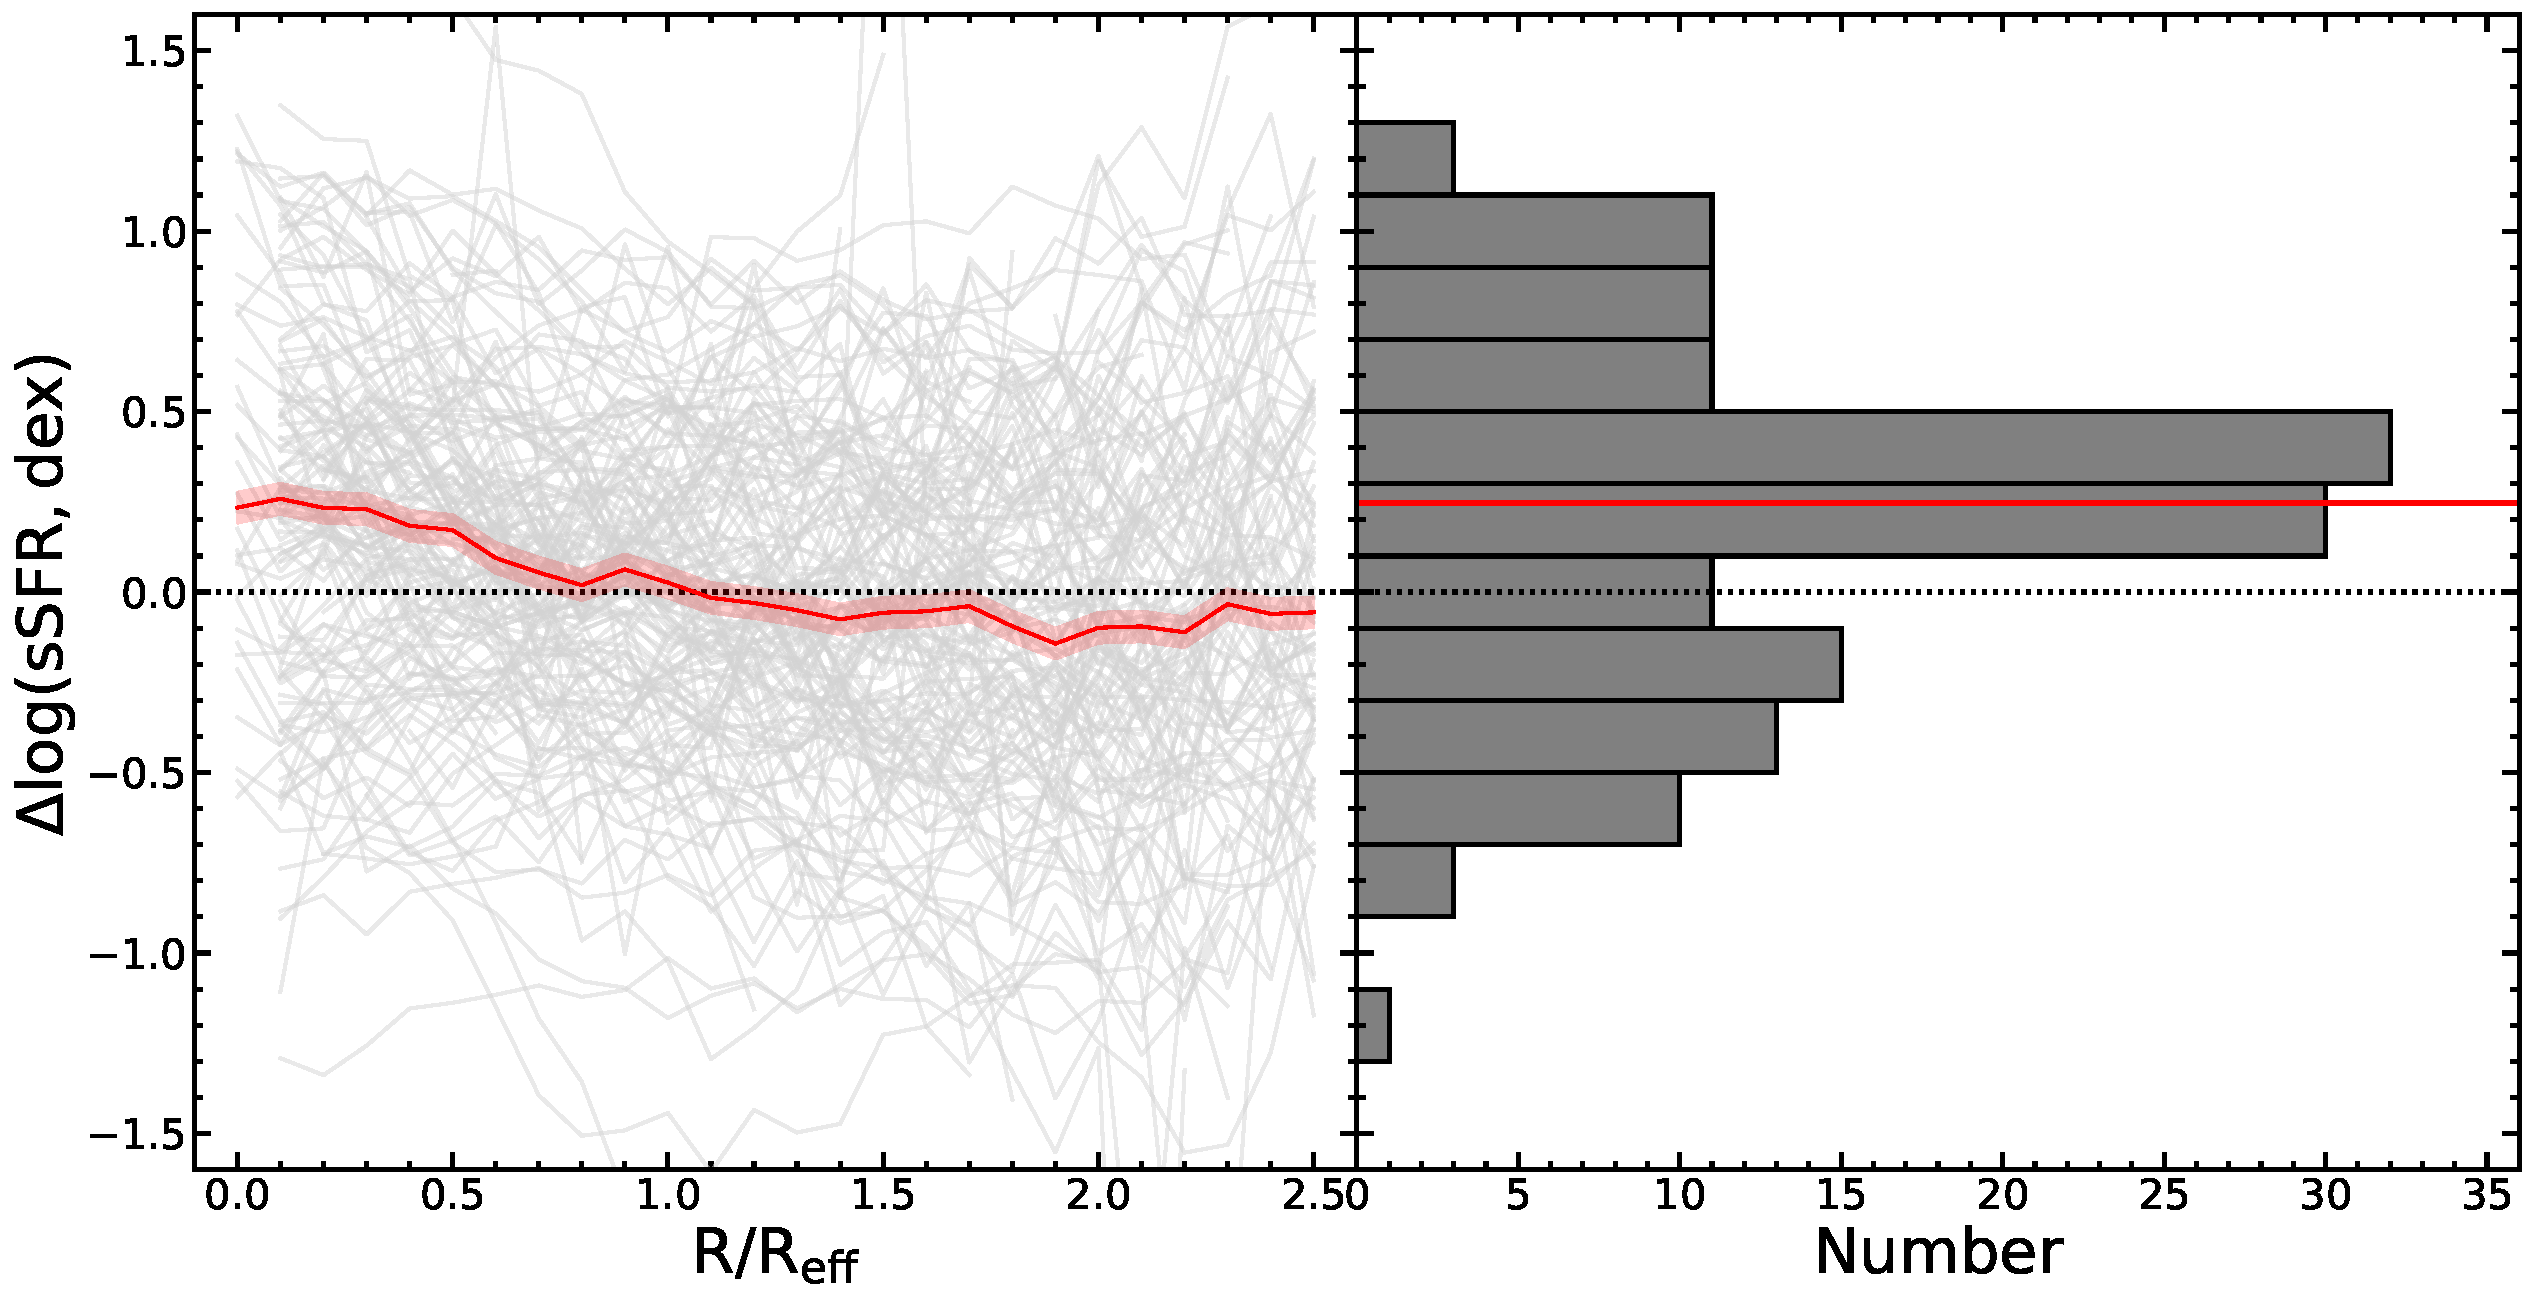
\includegraphics[width=\linewidth]{fig/ssfr_unsplit.pdf}
\caption[]{\textbf{Left:} The individual difference profiles are shown in light grey while the stacked profile for the whole pair sample is shown in red. The highlighted region about the profile is the standard error of the mean of the stacked profile. \textbf{Right:} A histogram of the $\delta$log(sSFR) within the inner 0.5 \reff\ of the individual difference profiles. The red line shows the median value of the $\Delta$log(sSFR) enhancement, $\sim$0.25 dex.}
\label{fig:ssfr_all}
\end{figure}
%%%%%%%%%%%%%%%%%%%%%%%%%%%%%%%%%%%%%%%%%%%%%%

We take each of the individual difference profiles for all of the and take the median value of the sSFR within each radius bin. This gives a single profile which describes the sSFR enhancements for the whole pair sample. We show this profile in the left hand panel of Figure \ref{fig:ssfr_all}. The sSFR is centrally enhanced by $\sim$0.25 dex. The enhancement falls to zero around 1.0\reff. The disks of the paired galaxies feature no enhancement or suppression to the sSFR. 

In the right hand panel of Figure \ref{fig:ssfr_all} we show a histogram for the $\Delta$log(sSFR) offset in the centers of the paired galaxies. To get this, we extract the values of $\Delta$log(sSFR) in the individual difference profiles within the inner 0.5 R/\reff\ and take the mean of the values. 

In the following sections we will break up the stacked profile into separate bins of total stellar mass, mass ratio, and projected separation. 

%%%%%%%%%%%%%%%%%%%%%%%%%%%%%%%%%%%%%%%%%%%%%%
\begin{figure*}
\centering
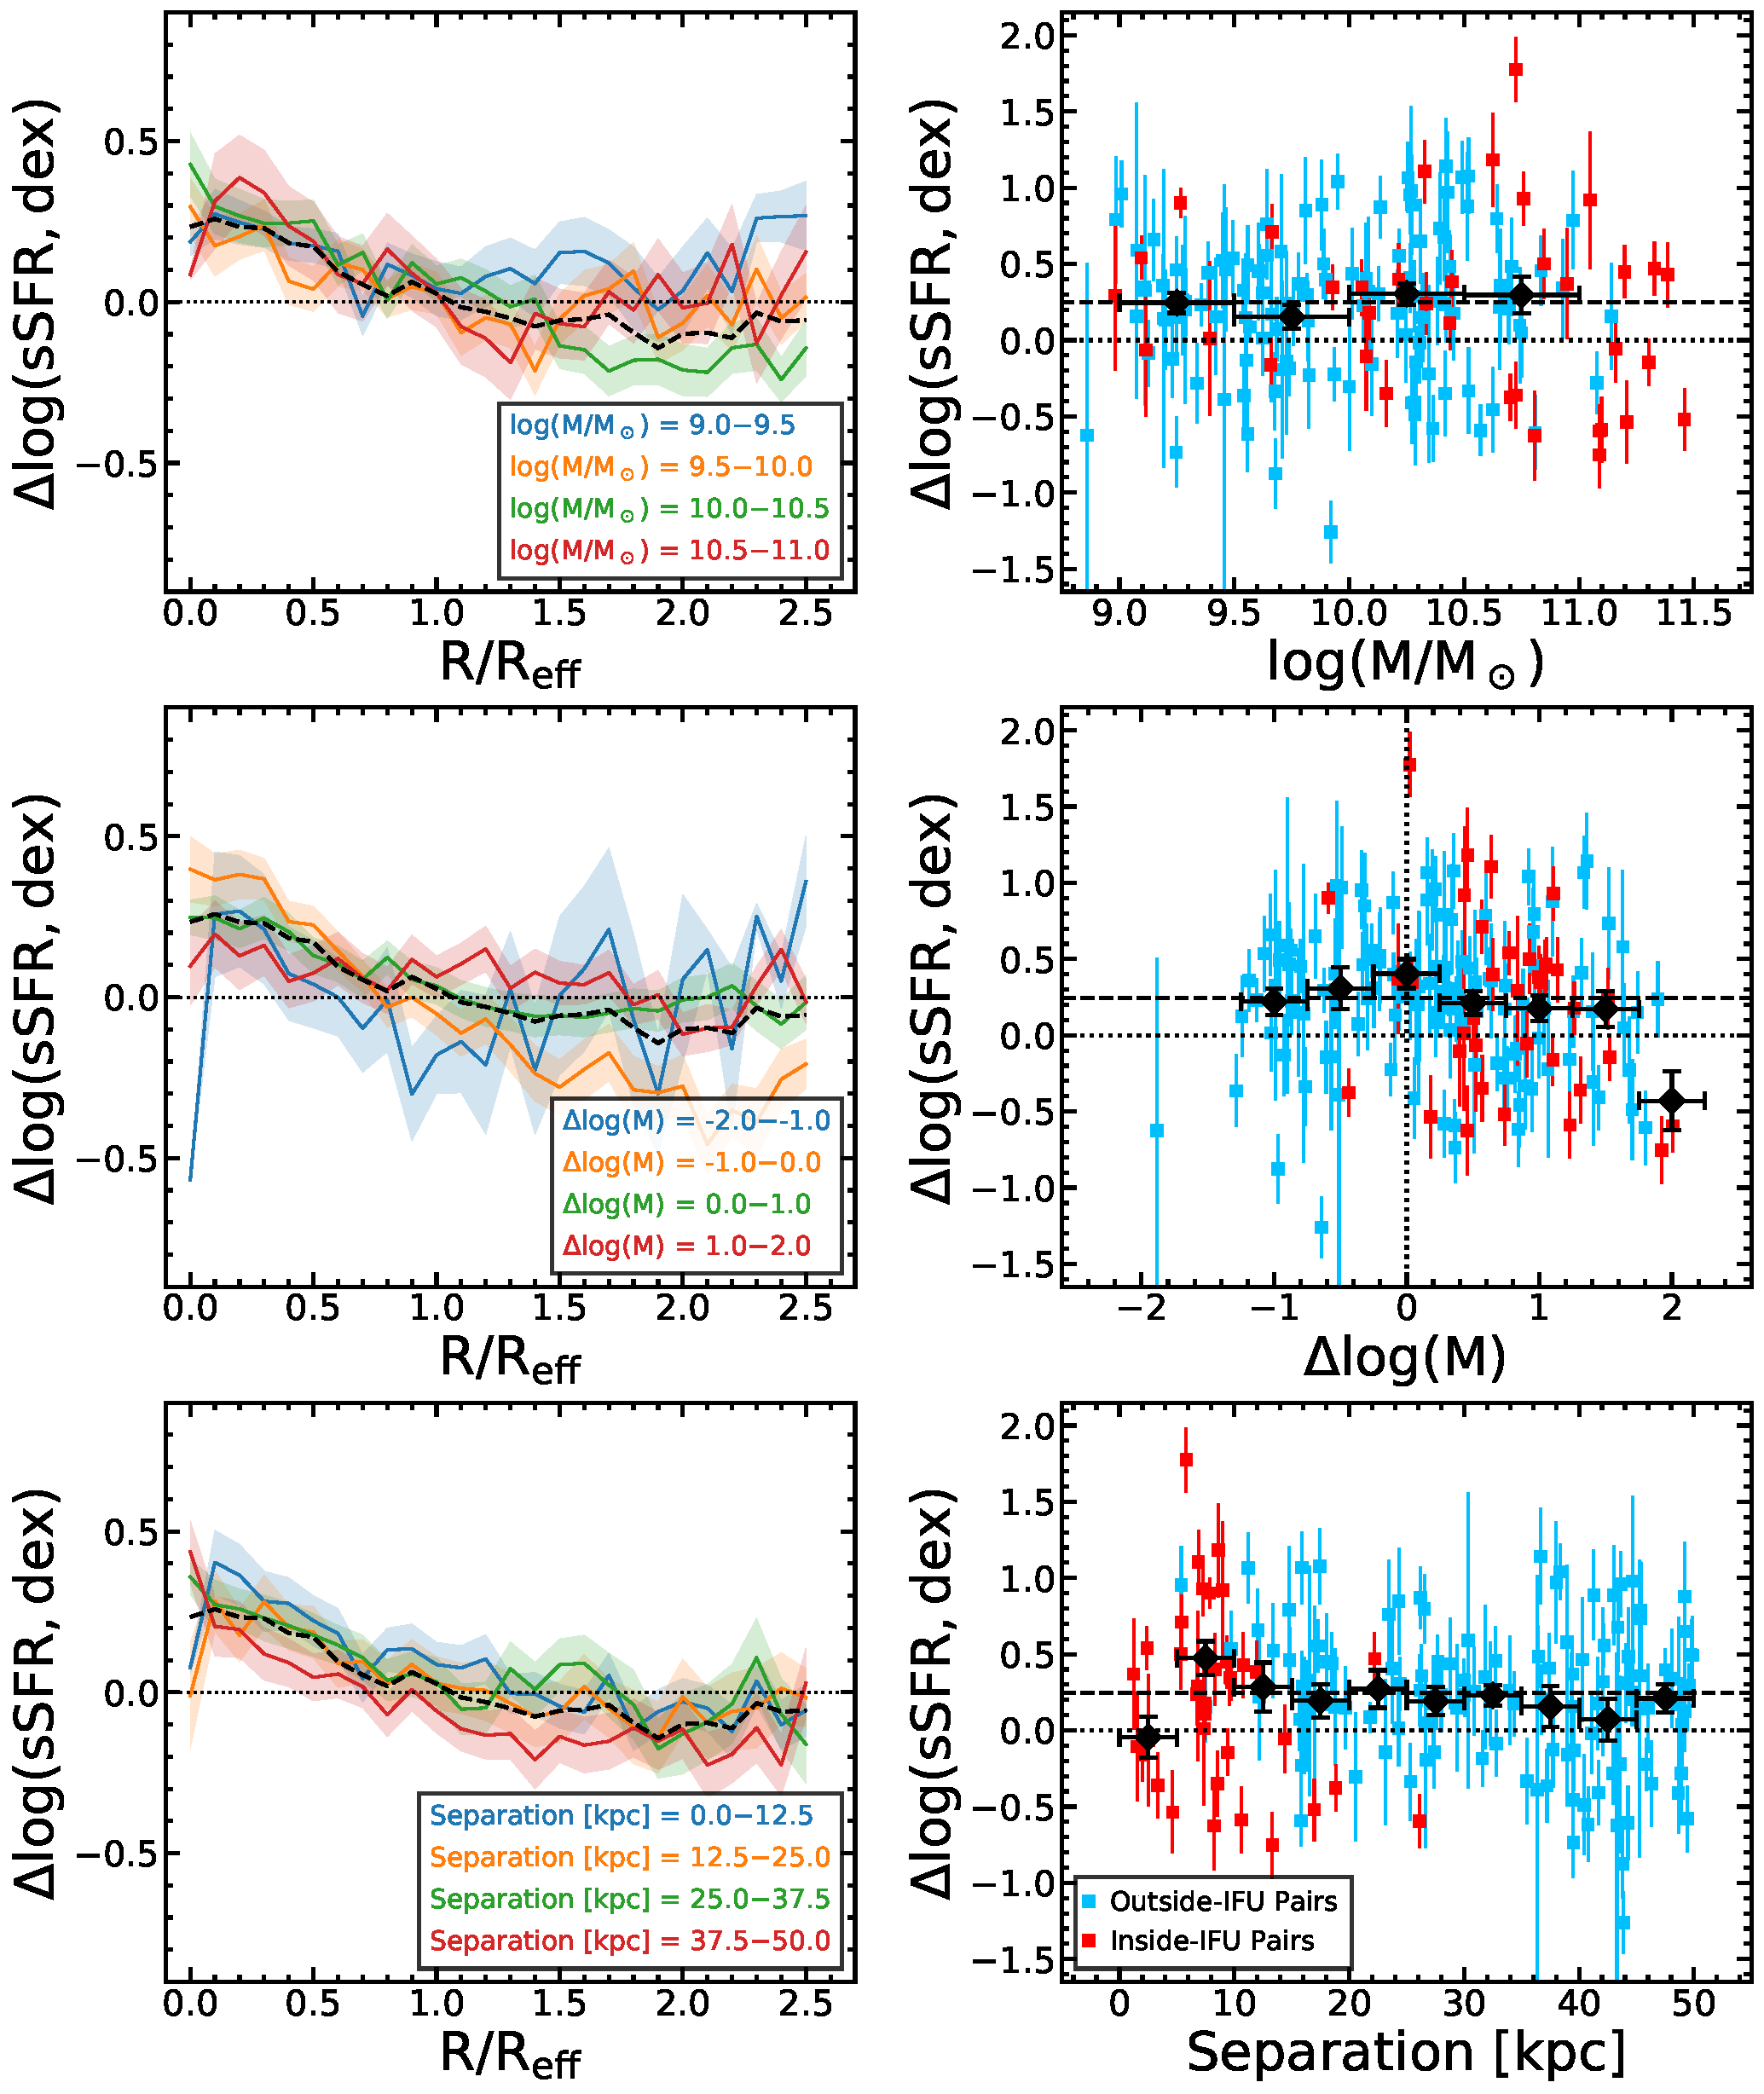
\includegraphics[width=\linewidth]{fig/ssfr_full.pdf}
\caption[]{The $\Delta$log(sSFR) split into separate stellar mass bins. The left column gives the stacked difference profiles. The highlighted region about the profiles represents the standard error of the mean of the profile. The black dashed line represents the stacked profile of the full pair sample. The right column gives the nuclear $\Delta$log(sSFR) values. The black squares are the mean values within a stellar mass bin (where the size of the bins are shown the the horizontal error bars). The vertical error bars on the black squares represent the standard deviation within the bin. The horizontal, dashed black lines represent the median central enhancement of the full pair sample. The top row shows the paired galaxies split by total stellar mass, the middle panel shows the paired galaxies split by mass ratio, and the bottom panel shows the paired galaxies split by projected separation. }
\label{fig:ssfr_full}
\end{figure*}
%%%%%%%%%%%%%%%%%%%%%%%%%%%%%%%%%%%%%%%%%%%%%%

\subsection{Stellar Mass}
We show the $\Delta$log(sSFR) profile split by the galaxy's total stellar mass in the top row of Figure \ref{fig:ssfr_full}. The level of the central sSFR enhancement is consistent with the level of enhancement for the full sample. This effect is better seen in the scatter plot of the central $\Delta$log(sSFR) offsets versus stellar mass where there is a flat distribution. 

In the disks of the paired galaxies, there is more scatter to the offsets of the profiles. The mass range, \logm\ $=$ 10.0$-$10.5, shows stronger suppression of sSFR in their disks while the mass range, \logm\ $=$ 9.0$-$9.5, show an enhancement to sSFR in their disks. There is no trend to sSFR enhancement/suppression with the stellar mass so the scatter in the profiles at large separation is likely due to a combination of the smaller sizes within separate mass bins and lower S/N at larger galactocentric radii.

From this we infer that the total stellar mass of a paired galaxy has no effect on the merger induced star formation within the galaxy. Massive galaxies are enhanced to the same degree as low mass galaxies. 

\subsection{Mass Ratio}
While the total stellar mass between the galaxies has no effect on the merger induced star formation, the mass ratio between the paired galaxies does. In the middle row of Figure \ref{fig:ssfr_full} we see that the sSFR enhancement is strongest in galaxies with mass ratios close to 1:1, $\delta$log(M) $=$ 0.0. These galaxies feature a central enhancement of $\sim$0.4 dex which is 0.15 dex higher than the average central enhancement of the whole sample. This enhancement falls with wider mass ratios and pairs with large differences in stellar mass still feature substantial levels of star formation enhancement, 0.2$-$0.25 dex at mass ratios of $|\Delta$log(M)$|$ $=$ 1.0.

We also use the mass ratio to explore how the merger induced tidal torques affect paired galaxies with large mass ratios, $|\Delta$log(M)$|$ > 0.5. We use the mass ratio to separate the massive central galaxy from satellite galaxies. A paired galaxy with a positive mass ratio is the more massive galaxy of the pair while a paired galaxy with negative mass ratio is the less massive galaxy. We see that the less massive galaxy of a pair show a higher level of sSFR enhancement, by $\sim$0.1 dex, with respect to the more massive galaxy. This shows us that satellite galaxies are more susceptible to tidal interactions than the central galaxies in the pair system. 

\subsection{Projected Separation}
Finally we look at the level of sSFR enhancement as a function of the projected separation between the two galaxies in the bottom row of Figure \ref{fig:ssfr_full}. The $\Delta$log(sSFR) profiles show a clear gradient with the projected separation where close galaxy pairs show higher levels of sSFR enhancement compared to pairs with wide separations. 

This effect can be seen most clearly in the scatter plot of the central $\Delta$log(sSFR) enhancement as a function of projected separation. The level of the enhancement gradually increases with closer separation from 50 kpc to 10 kpc. Within 10 kpc, the $\Delta$log(sSFR) enhancement jumps to 0.5 dex. Surprisingly, this central enhancement plummets back to zero at the closest separations, r$_p$ $<$ 5 kpc. We will discuss the potential causes of the zero enhancement in the centers of the closest galaxies in Section \ref{sec:discussion}.

\subsection{Future Mass Growth}
%%%%%%%%%%%%%%%%%%%%%%%%%%%%%%%%%%%%%%%%%%%%%%
\begin{figure*}
\centering
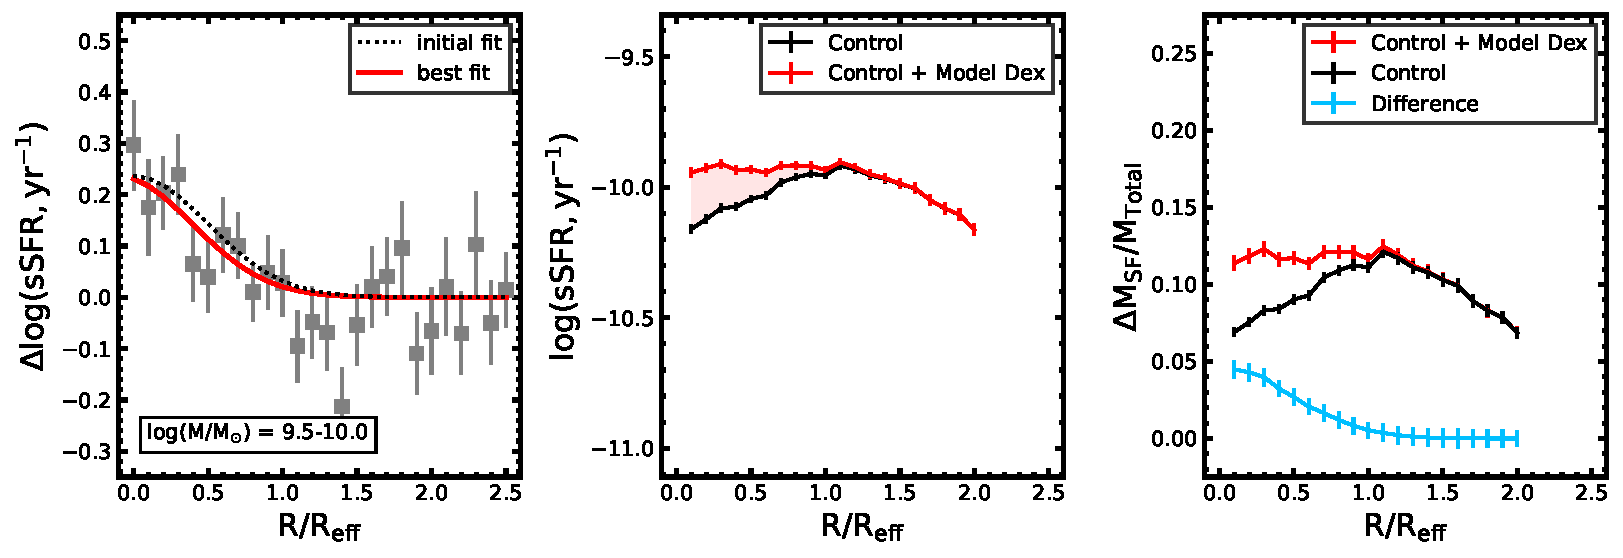
\includegraphics[width=\linewidth]{fig/mass_gain_1.pdf}
\caption[Example of the calculation of the fractional mass gain due to merger induced star formation for a single mass bin.]{In the Left panel we fit a model gaussian to the $\Delta$log(sSFR) profiles. In the Middle panel we plot the log(sSFR) profile for the stacked profiles of the control galaxies (black). We then add the modeled $\Delta$log(sSFR) profile to the control profile (red). The error bars represent the standard error of the mean of the profiles. In the Right panel we show the fractional mass gain due to star formation in the control galaxies (black) and in the paired galaxies (red). The blue profile is the subtraction between the pairs and controls and represents the fractional mass gain due to merger induced star formation. The error bars represent the standard error of the mean of the profiles. }
\label{fig:mass_gain}
\end{figure*}
%%%%%%%%%%%%%%%%%%%%%%%%%%%%%%%%%%%%%%%%%%%%%%

%%%%%%%%%%%%%%%%%%%%%%%%%%%%%%%%%%%%%%%%%%%%%%
\begin{figure}
\centering
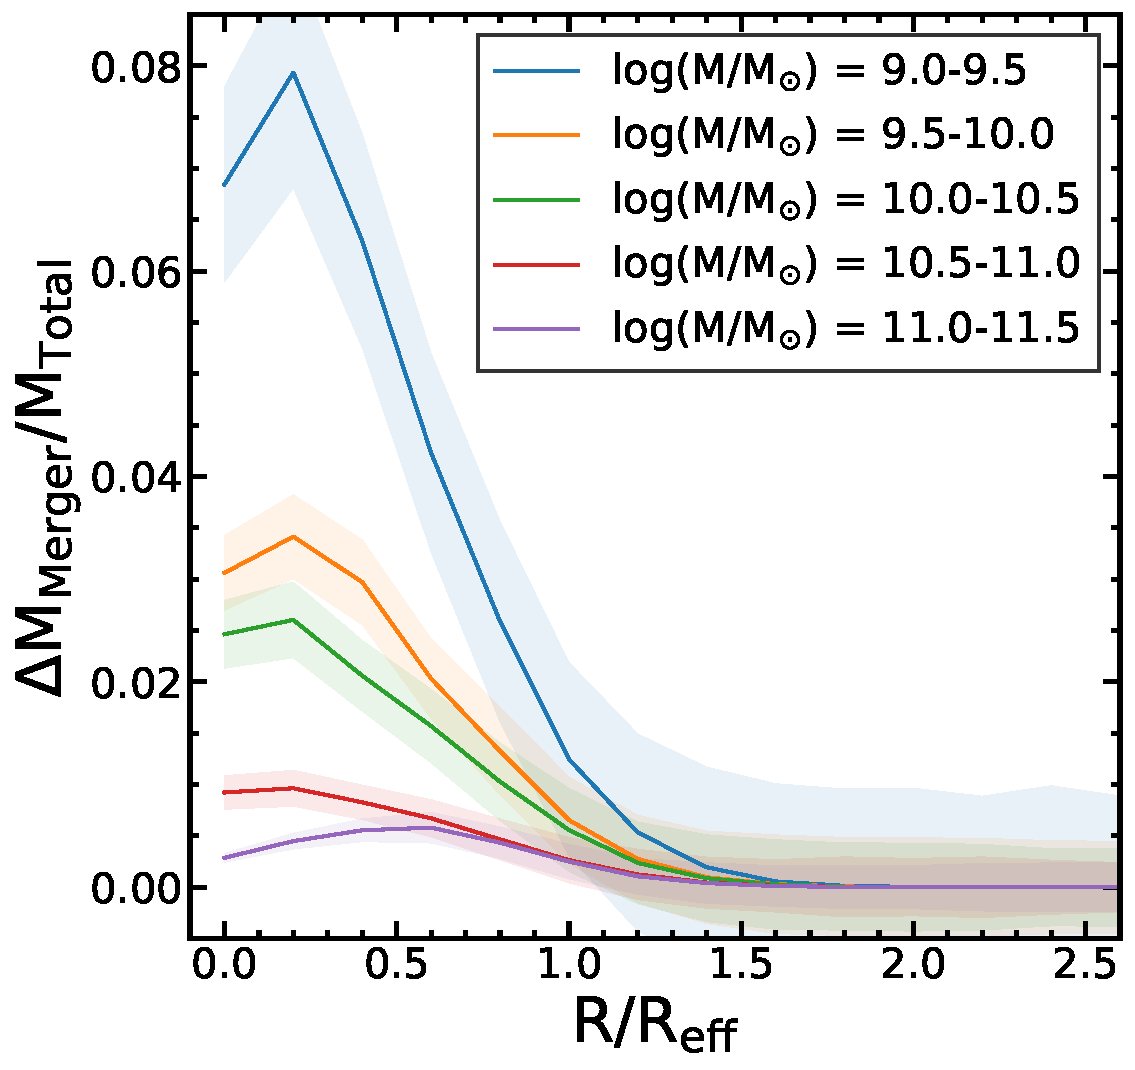
\includegraphics[width=3in]{fig/mass_gain.pdf}
\caption[The fractional mass gain due to merger induced star formation.]{The fractional mass gain due to merger induced star formation over a dynamical timescale, $\tau$ $=$ 1 Gyr. The highlighted region represents the propagated standard errors of the mean of the stacked log(sSFR) profiles. }
\label{fig:mass_gain_sum}
\end{figure}
%%%%%%%%%%%%%%%%%%%%%%%%%%%%%%%%%%%%%%%%%%%%%%

The merger induced star formation will increase the mass growth rate of the interacting galaxies. We will use a simple model to estimate the enhanced mass growth rate due to merger induced star formation. 

A specific star formation rate is already a representation of the fractional mass growth every year, so the merger induced mass growth is simply;

\begin{equation}
\frac{\Delta M_{merger}}{M_{total}} = \left(sSFR_{pair} - sSFR_{control}\right) * \tau_{dyn}
\end{equation}

Where $\tau_{dyn}$ is the dynamical timescale of the merger event. For this estimation we use a timescale of 1 Gyr, which is the order of the typical timescale between the passage of the first and second pericenters in hydrodynamical simulations \citep{Boylan-Kolchin:2008}. 

To get the difference in sSFR between the pairs and controls, we fit a gaussian to the difference profiles split by stellar mass. We then add the modeled difference profile to the stacked control profile in the same mass range in log space. We then take the difference between the profiles in linear space and multiple the difference by the 1 Gyr timescale. This process is shown for a single mass range in Figure \ref{fig:mass_gain}.

We show the mass growth rate profile for each of the four mass ranges in Figure \ref{fig:mass_gain_sum}. The mass growth rate is largely restricted to the centers of the galaxies, following the centrally enhanced sSFR. The mass growth rate is strongly dependent on the stellar mass of the paired galaxies. 

The fractional mass change is greatest in the less massive galaxies, $\Delta$M$_{merger}$/M$_{total}$ $=$ 0.065, while it is less substantial is the more massive galaxies, $\Delta$M$_{merger}$/M$_{total}$ $=$ 0.015. This is unsurprising as the $\Delta$log(sSFR) profiles were independent of the galaxies' total stellar mass. 

Galaxies in the mass range \logm\ $=$ 9.0$-$10.0 have a mass growth of $\sim$1.6$\times$ that of secular mass growth and galaxies in the mass range \logm\ $=$ 10.0$-$11.0 have a mass growth of $\sim$2.3$\times$ that of secular mass growth. While low mass galaxies may see a more substantial change to their total stellar mass, the more massive galaxies experience higher growth rates.

%%%%%%%%%%%%%%%%%%%%%%%%%%%%%%%%%%%%%%%%%%%%%%%%%%%%
\section{Discussion}\label{sec:discussion}


%%%%%%%%%%%%%%%%%%%%%%%%%%%%%%%%%%%%%%%%%%%%%%%%%%%%
\section{Summary and Conclusion}\label{sec:sum}






\acknowledgments

% funding
J.S. and H.F. acknowledge support from the National Science Foundation (NSF) grant AST-1614326 and University of Iowa funds. 

%%%%%%%%%%%%%%%%%%%% REFERENCES %%%%%%%%%%%%%%%%%%
\bibliographystyle{aasjournal}
\bibliography{mergerbib}

%%%%%%%%%%%%
% Appendix
%%%%%%%%%%%%

\hbox{}\clearpage

\appendix

\section{Figures}

%%%%%%%%%%%%%%%%%%%%%%%%%%%%%%%%%%%%%%%%%%%%%%
\begin{figure}
\centering
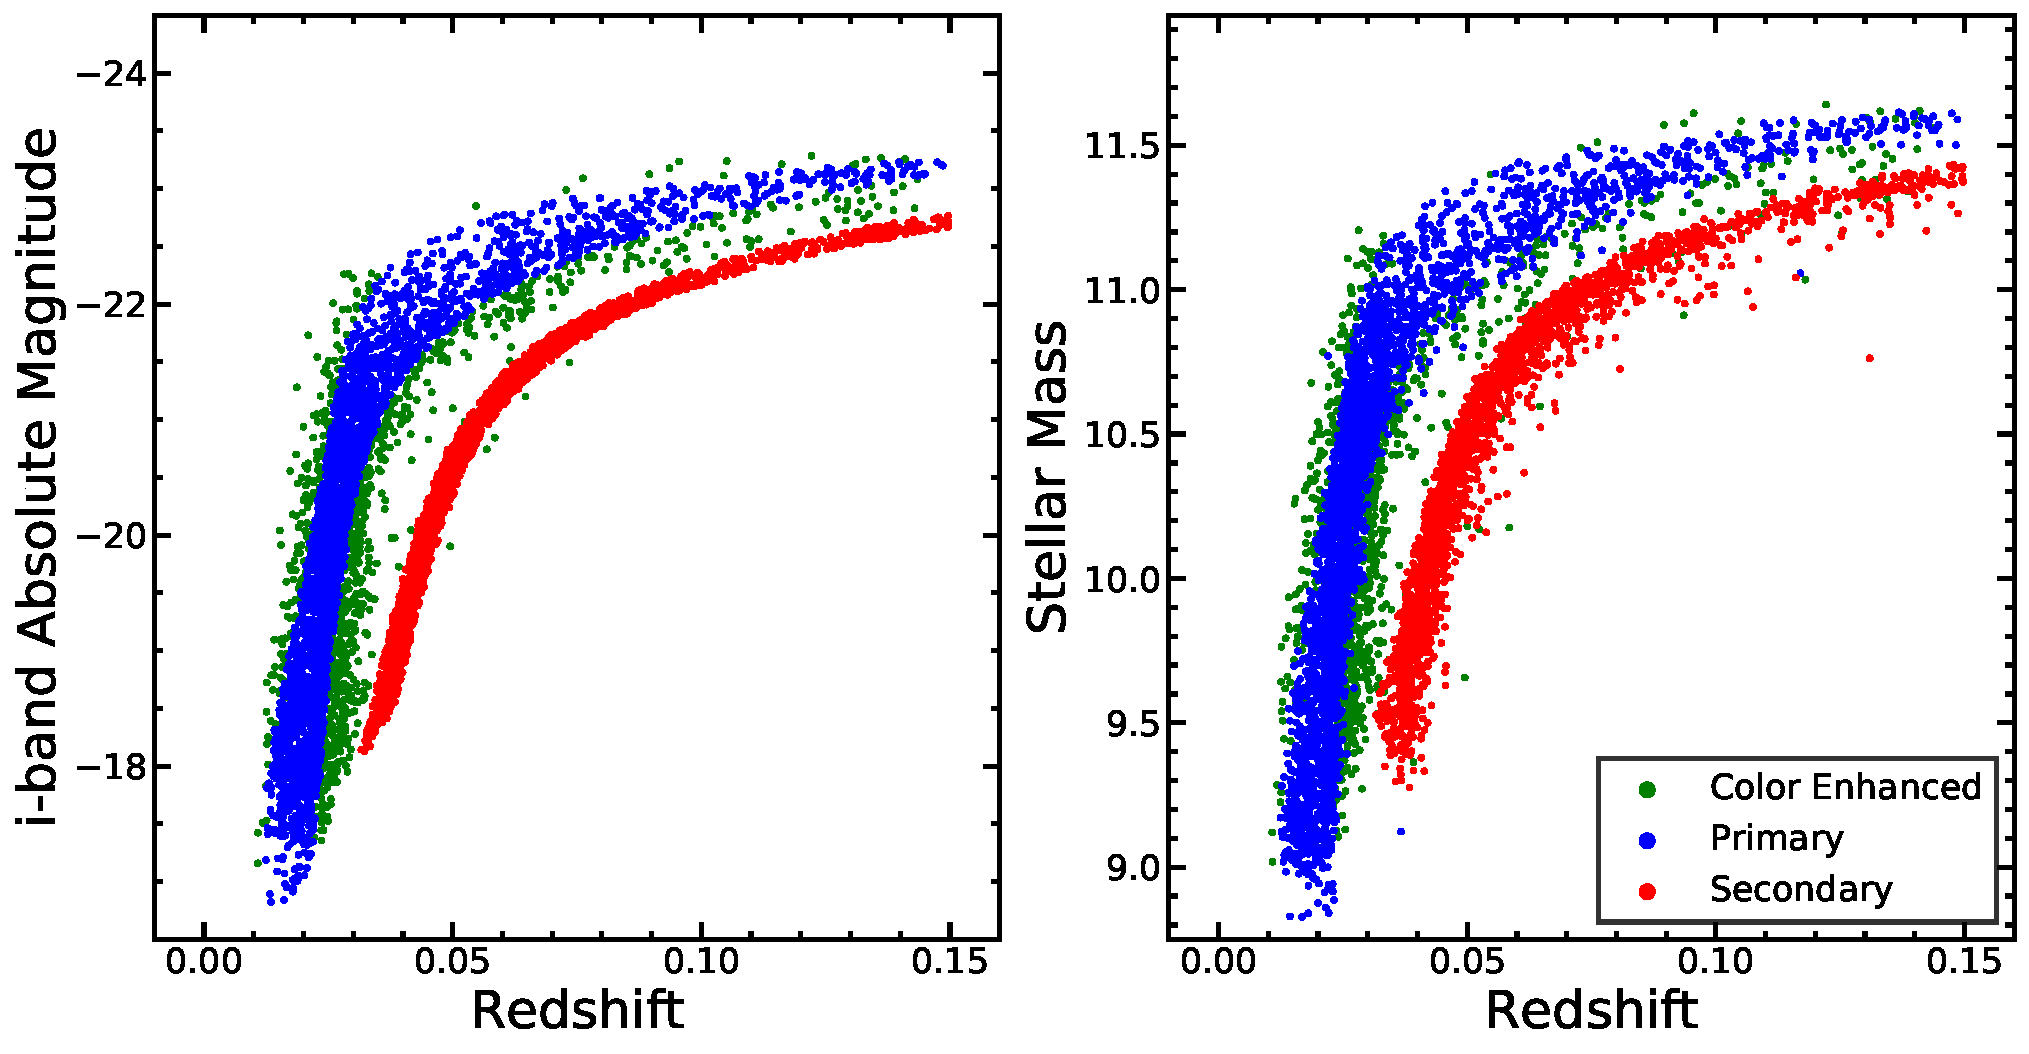
\includegraphics[width=\linewidth]{fig/Mi-z.pdf}
\caption[The luminosity - redshift distribution and mass - redshift distribution of the MaNGA sample.]{On the left is the luminosity - redshift distribution of the MaNGA sample. The figure illustrates the unique distribution of the MaNGA sample. On the right, I replace the luminosity with stellar mass from the NSA catalog.}
\label{fig:Mi-z}
\end{figure}
%%%%%%%%%%%%%%%%%%%%%%%%%%%%%%%%%%%%%%%%%%%%%%

%%%%%%%%%%%%%%%%%%%%%%%%%%%%%%%%%%%%%%%%%%%%%%
\begin{figure}
\centering
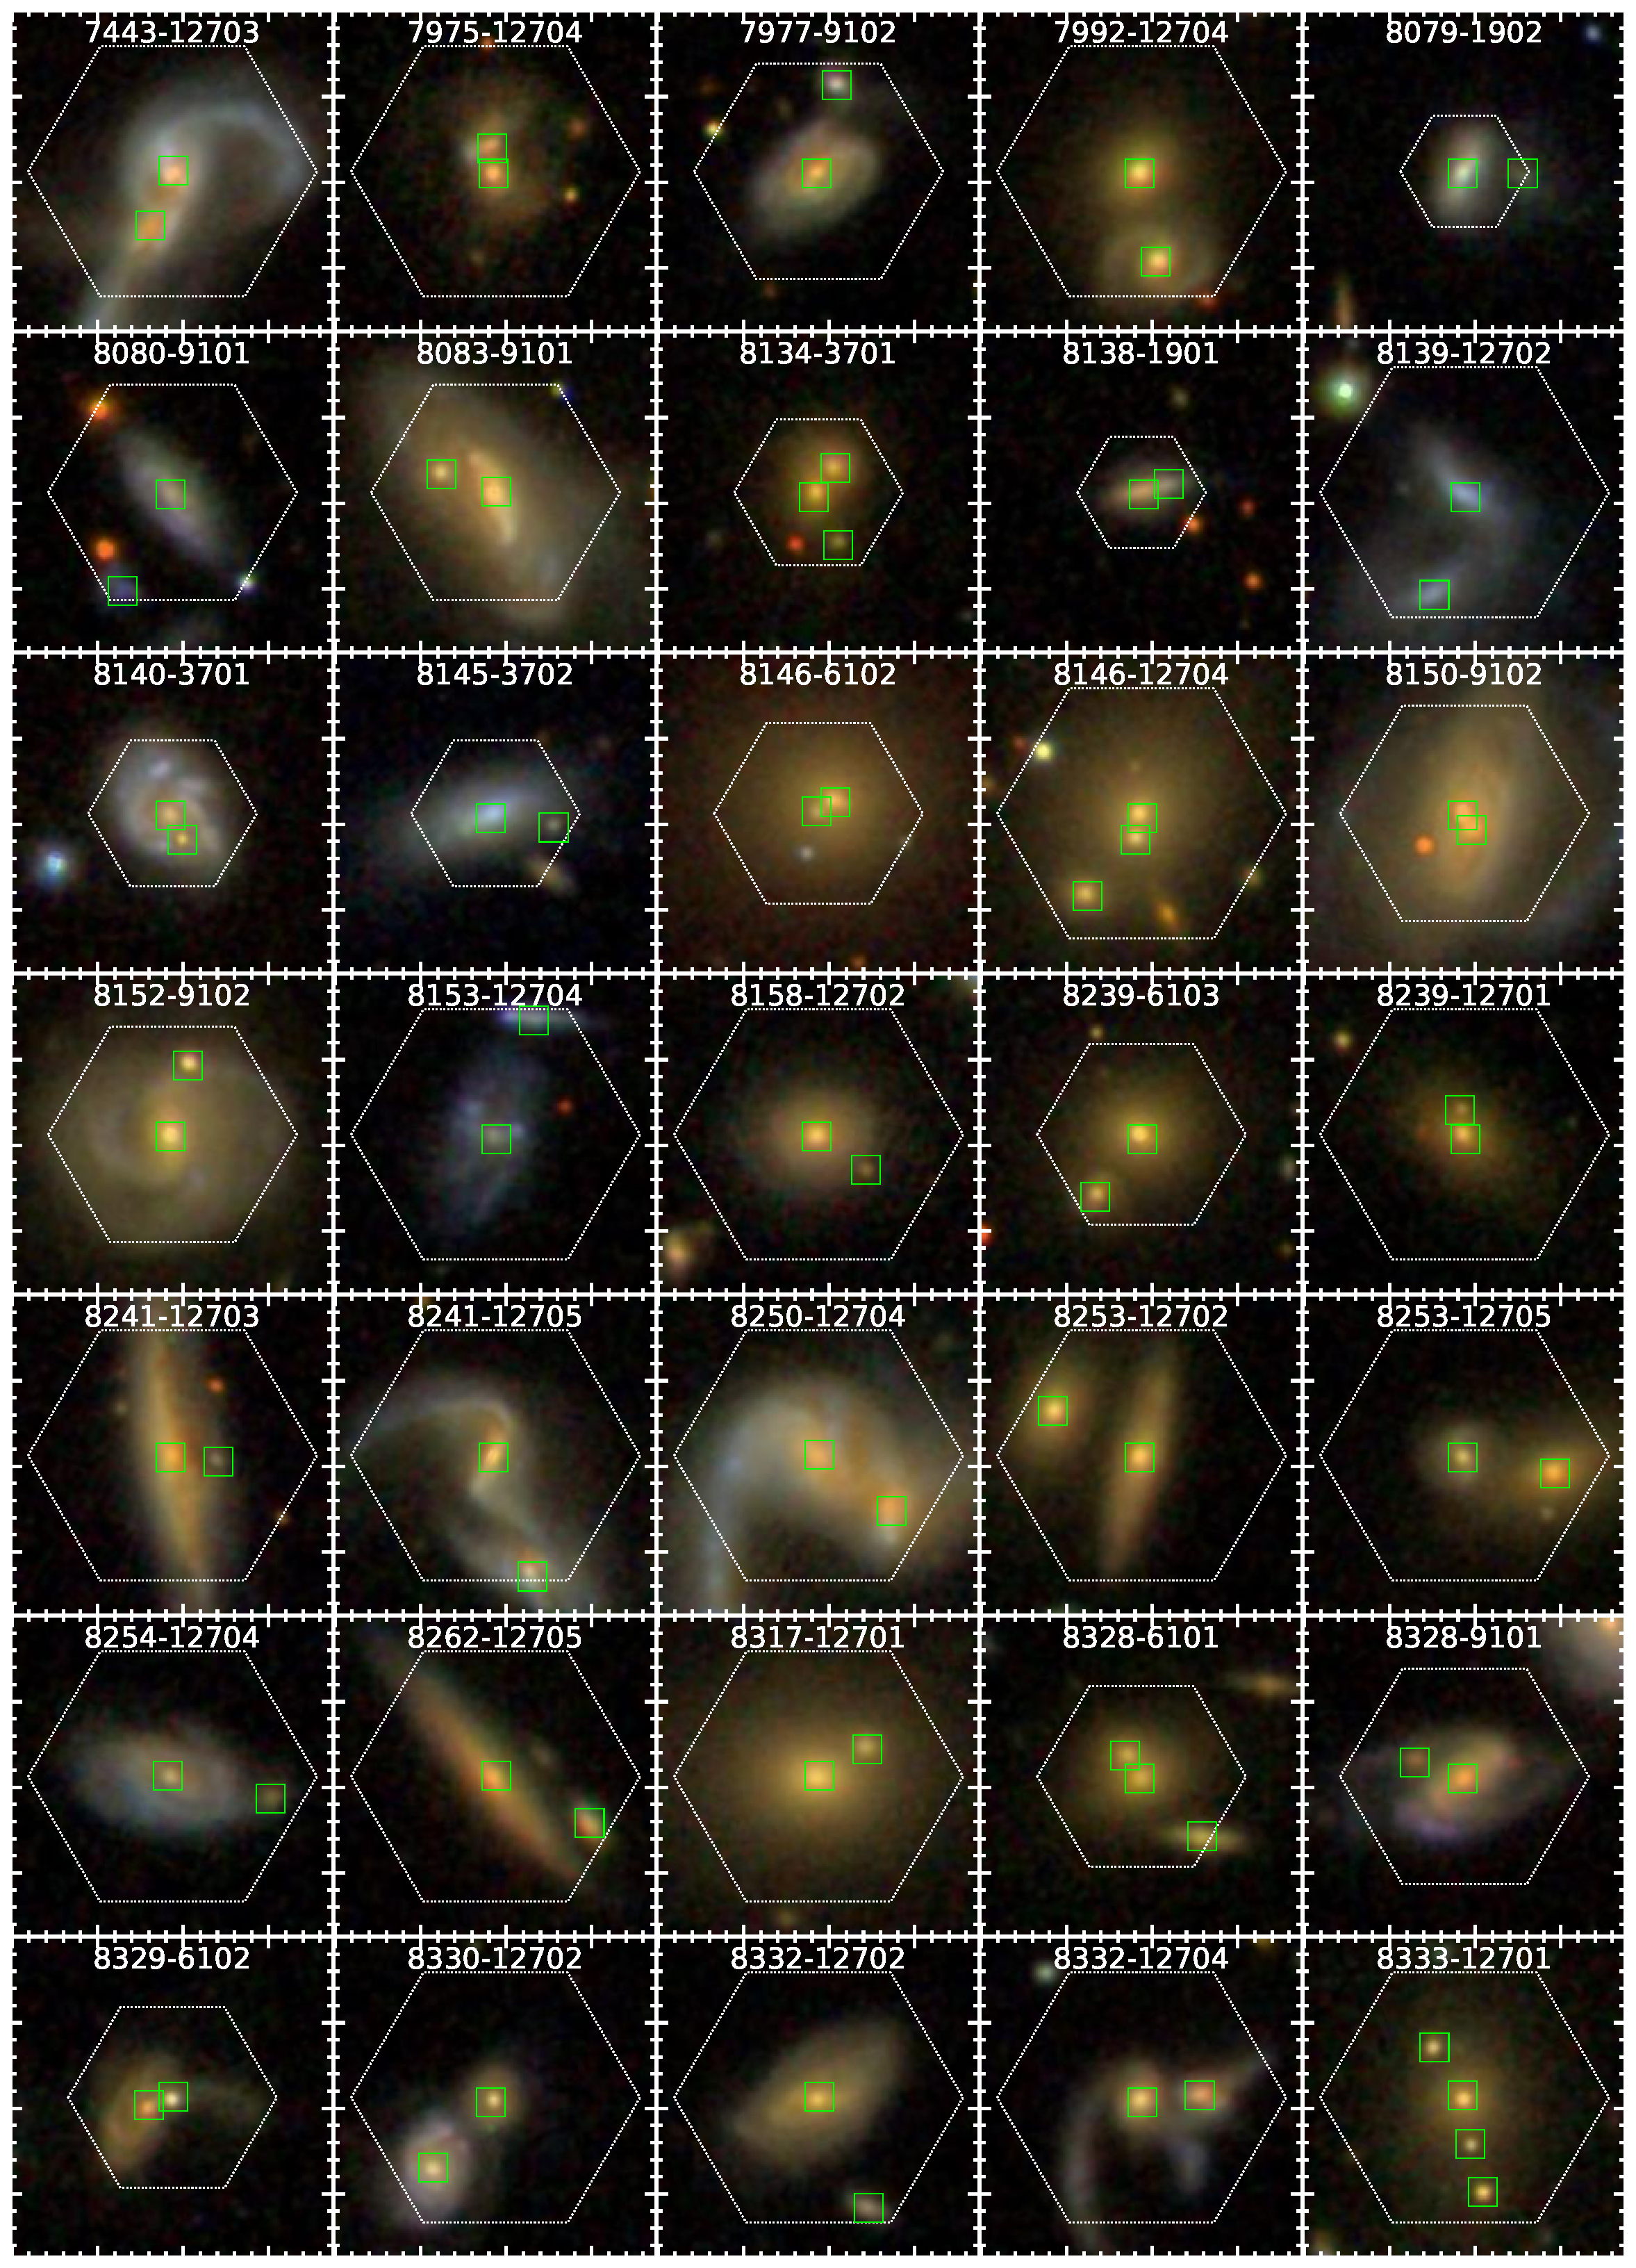
\includegraphics[width=\linewidth]{fig/pair_collage.pdf}
\caption[A collage of a subset of the inside-IFU pairs.]{A collage of a subset of the inside-IFU pairs. Each panel contains a 40$^{\arcsec}$ cutout of the SDSS pseudocolor image for the galaxy pair. The minor ticks on each panel's axis represents 2$^{\arcsec}$. The green squares highlight the identified galaxy pairs. }
\label{fig:collage}
\end{figure}
%%%%%%%%%%%%%%%%%%%%%%%%%%%%%%%%%%%%%%%%%%%%%%

%%%%%%%%%%%%%%%%%%%%%%%%%%%%%%%%%%%%%%%%%%%%%%
\begin{figure*}
\centering
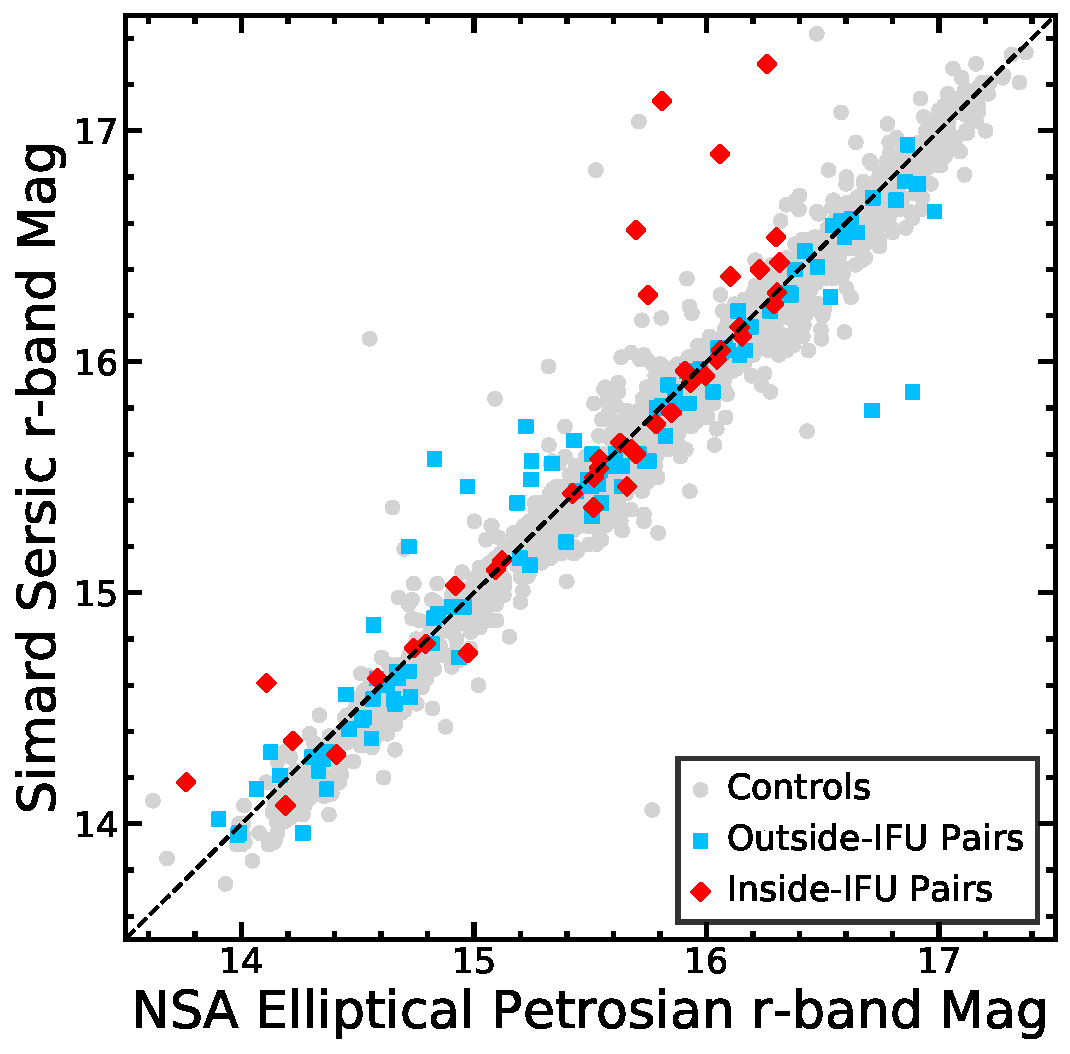
\includegraphics[width=3in]{fig/mag_comp.pdf}
\caption[The comparison between the r-band magnitudes in Simard+11 and NSA catalog]{The comparison between the S\'ersic r-band apparent magnitude in \citet{Simard:2011} and the Elliptical Petrosian r-band apparent magnitude. The grey circles represent galaxies in the control sample, the blue squares represent galaxies in the outside-IFU sample, and the red diamonds represent the galaxies in the inside-IFU sample. Regardless of the sample, all of the galaxies covered by both of the catalogs have a similar apparent magnitude calculated from either sample.}
\label{fig:mag_comp}
\end{figure*}
%%%%%%%%%%%%%%%%%%%%%%%%%%%%%%%%%%%%%%%%%%%%%%

%%%%%%%%%%%%%%%%%%%%%%%%%%%%%%%%%%%%%%%%%%%%%%
\begin{figure*}
\centering
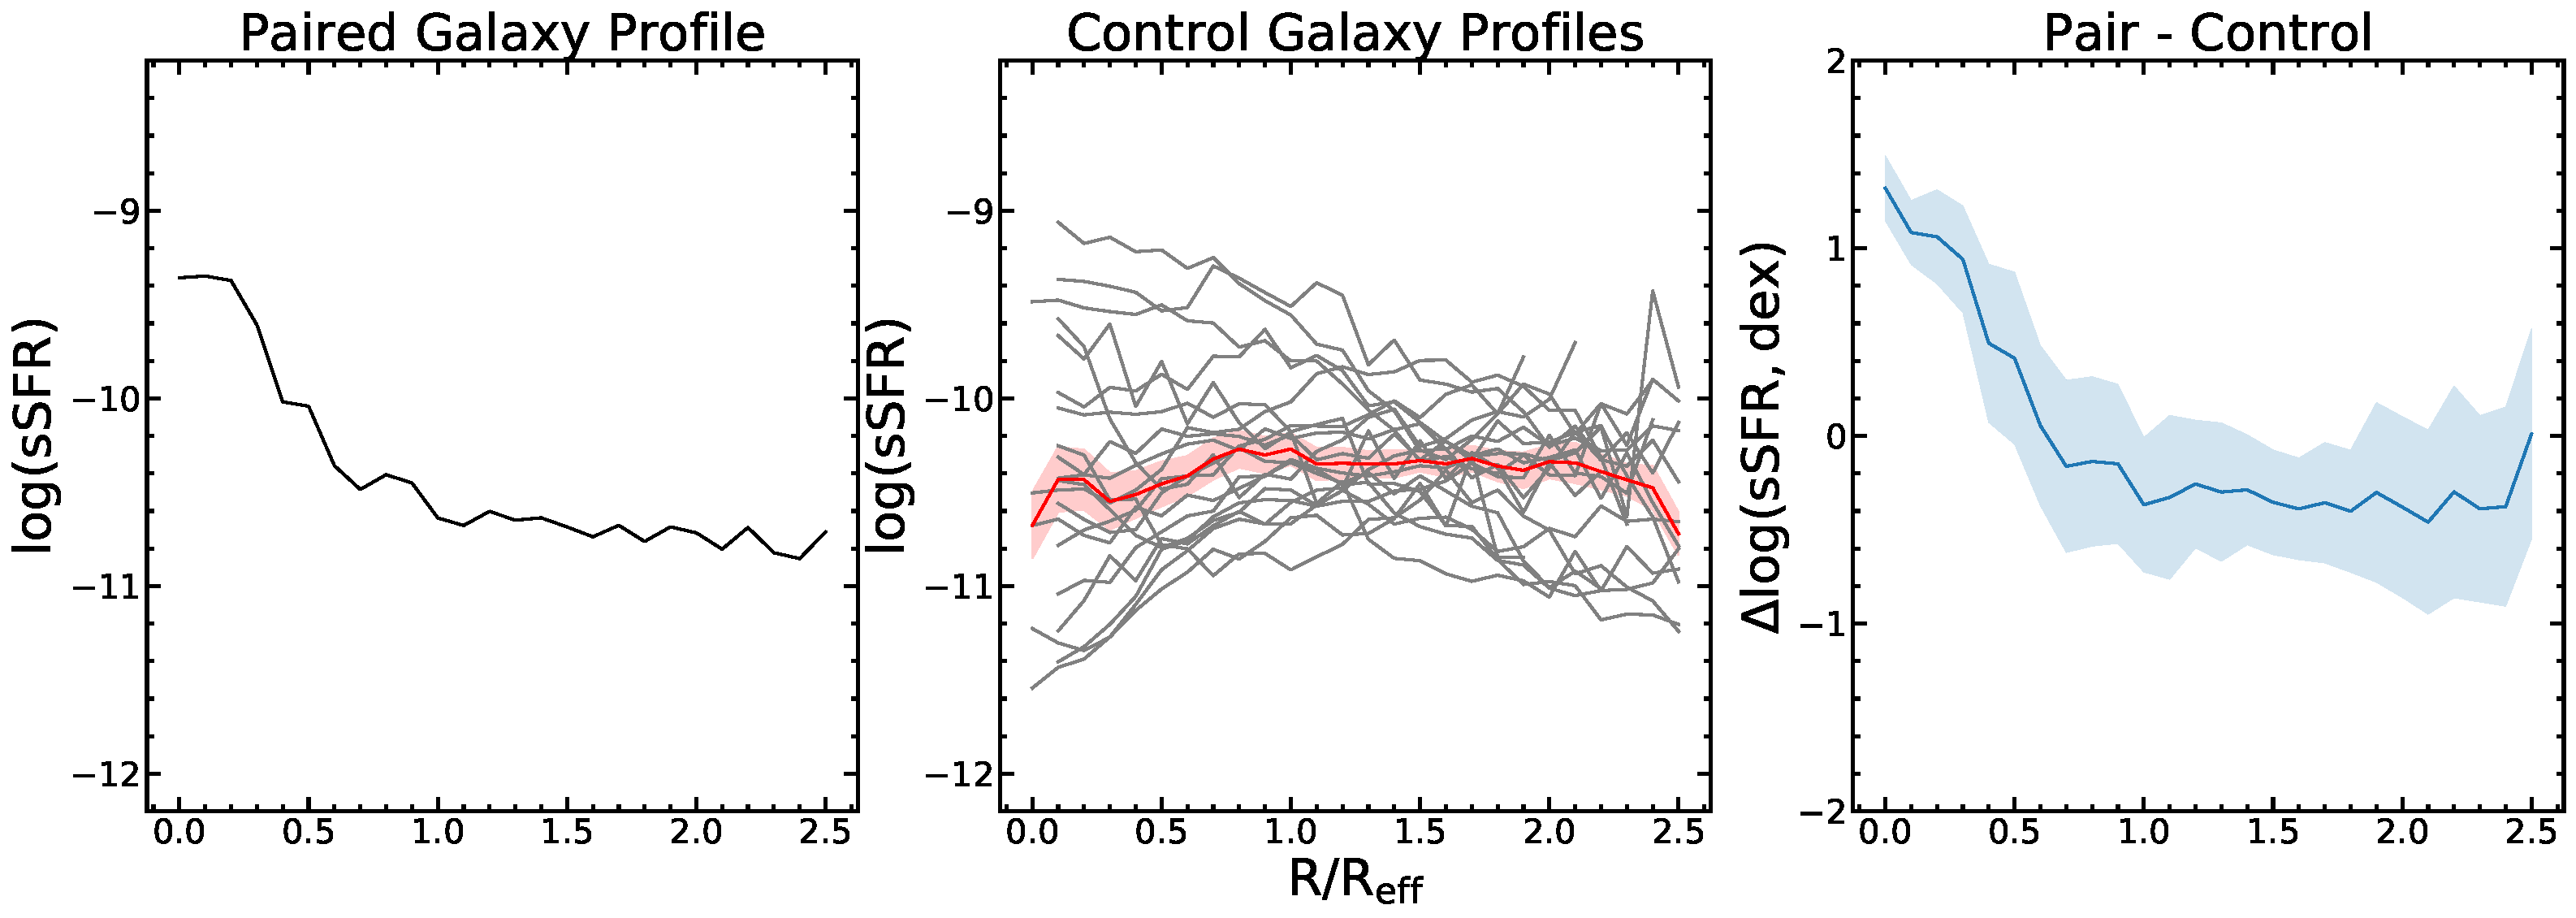
\includegraphics[width=\linewidth]{fig/8083-12703.pdf}
\caption[Example of the difference profiles for the mass-redshift selected control sample.]{The process for building the tailored control sample. The Left panel shows the paired galaxy's profile for sSFR. The Middle panel shows the profiles for sSFR for the selected 20 control galaxies in gray. The red profile is the median profile of the 20 control galaxies where the highlighted region about the profile is the standard error of the mean. The Right panel shows the difference between pair's profile and the stacked control profile.}
\label{fig:dex}
\end{figure*}
%%%%%%%%%%%%%%%%%%%%%%%%%%%%%%%%%%%%%%%%%%%%%%

%%%%%%%%%%%%%%%%%%%%%%%%%%%%%%%%%%%%%%%%%%%%%%
\begin{figure*}
\centering
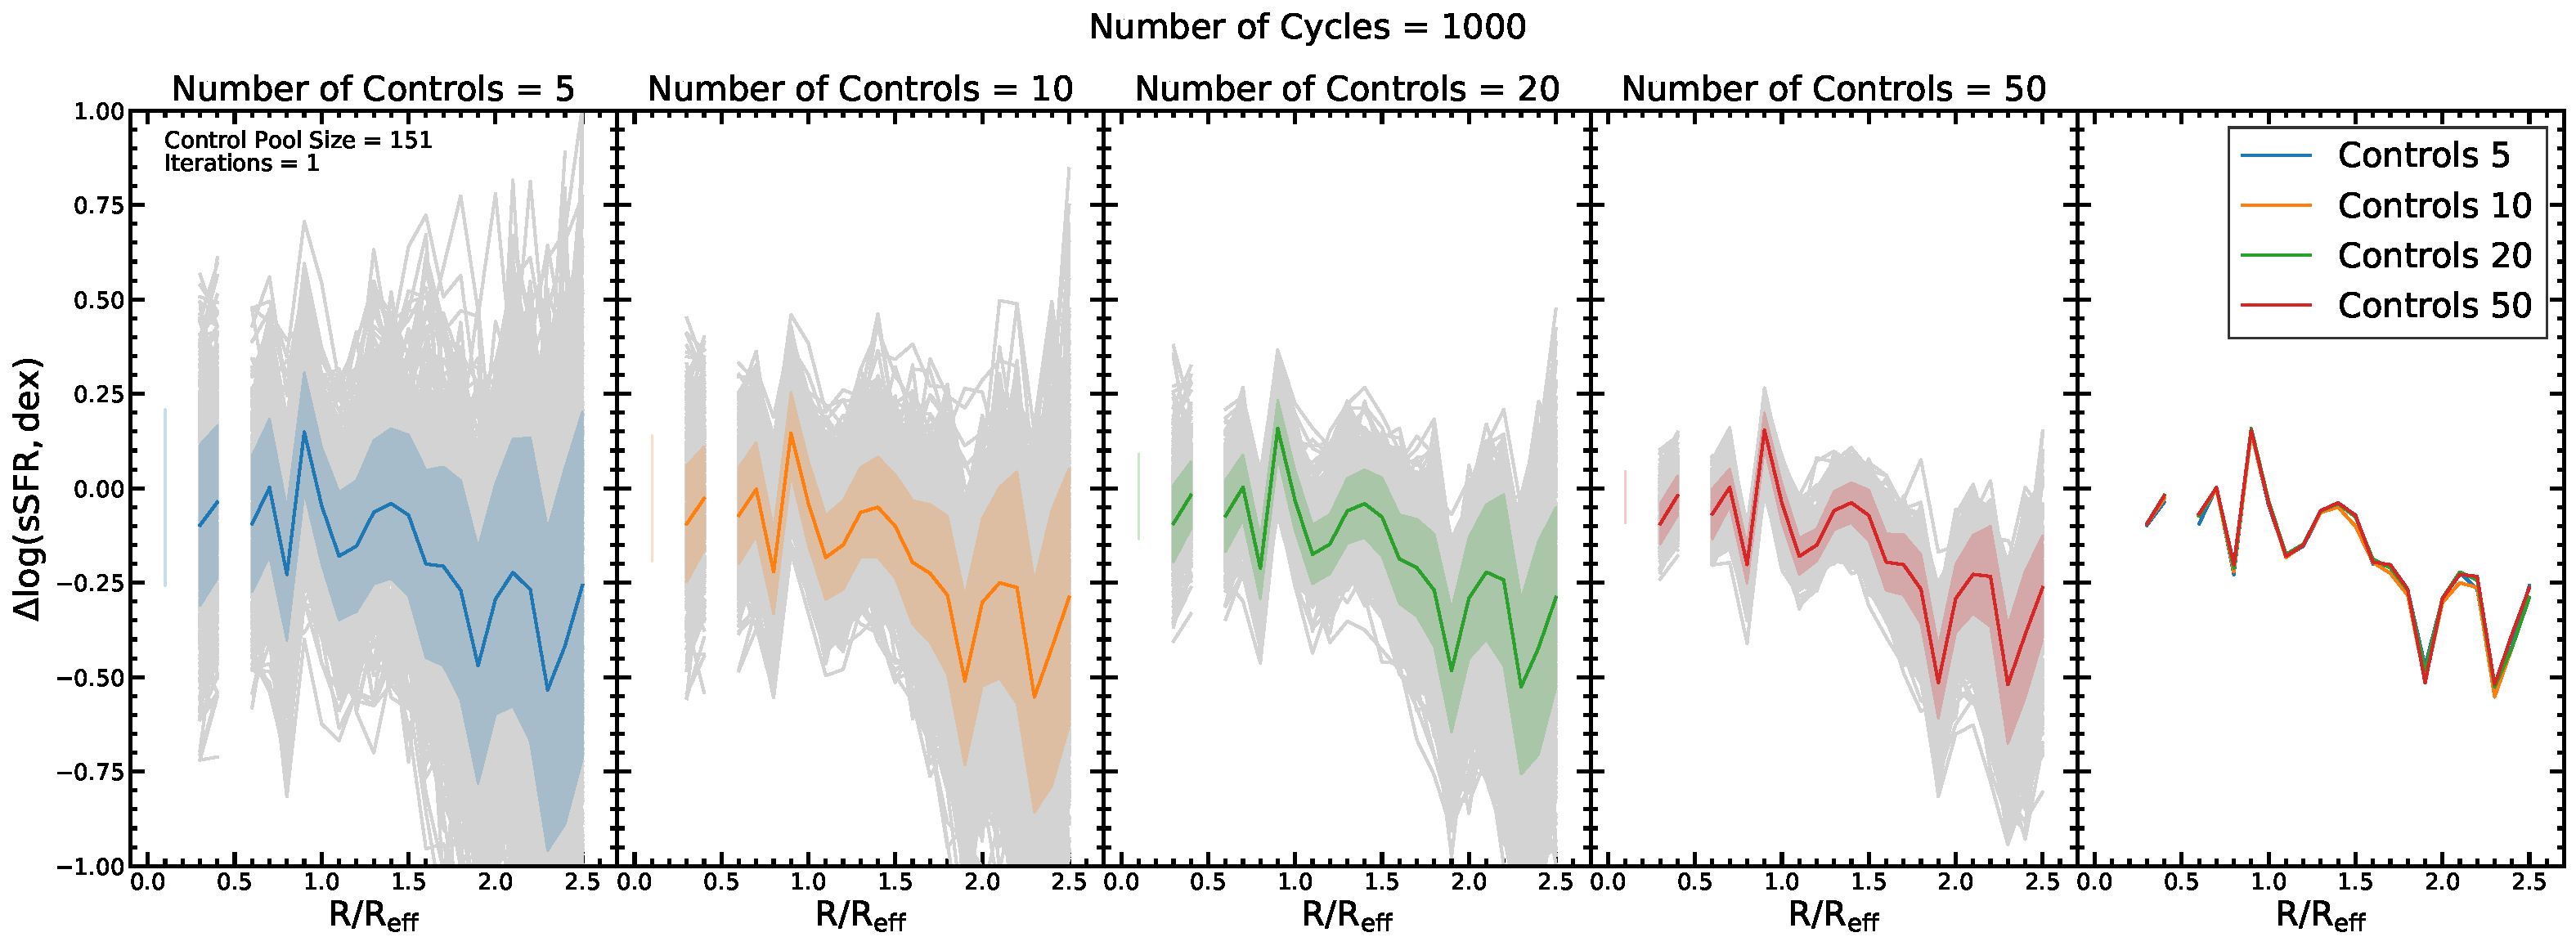
\includegraphics[width=\linewidth]{fig/8485-3704.pdf}
\caption[Example of bootstrapping to quantify the deviation of the random subsample of controls]{An example of the bootstrapping used to quantify the errors associated with the random selection of the control subsample. From left to right, the first four panels show the individual dex profiles after a random sub-selection in grey. The random sub-selection is run 1000 times and the median profile after the 1000 cycles is given by the colored profile. The highlighted region about the colored profiles is the standard error of the mean of the median profile. From left to right each panel shows the random selection for a different number of controls to select; 5, 10, 20, and 50 controls. The panel on the right end shows the median profiles of all of the preceding panels. }
\label{fig:bootstrap}
\end{figure*}
%%%%%%%%%%%%%%%%%%%%%%%%%%%%%%%%%%%%%%%%%%%%%%

\end{document}